\chapter{Arhitektura i dizajn sustava}

		Arhitektura programske potpore predstavlja strukturu sustava ili više njih koje sadrži elemente, njihova obilježja i odnose među njima. Temeljni razlozi definiranja arhitekture:		

	\begin{itemize}
		\item 	{poboljšava razumljivost i komunikaciju sudionika}
		\item 	{pomaže u donošenju temeljnih odluka pri izradi projekta}
		\item 	{omogućava rano uočavanje pogrešaka u oblikovanju}		
		\item         {moguće ponovno korištenje rješenja (engl. reuse)}
	\end{itemize}

	U konačnici, efikasno strukturiranje arhitekture programske potpore dovest će do poboljšanja kvalitete finalnog produkta projekta.

	\vspace{10mm} %10mm vertical space

	Koristimo objektno usmjerenu arhitekturu koja najbolje odgovara razvoju složene Web aplikacije namijenjene za što više korisnika u stvarnom vremenu. Možemo ju klasificirati na četiri ključna dijela koji osiguravaju izvršavanje naredbi korisnika: 
		
	\begin{packed_enum}
		\item 	{Web preglednik}
		\item 	{Web poslužitelj}
		\item 	{Web aplikacija}
		\item 	{Baza podataka}
	\end{packed_enum}			

		\begin{figure}[H]
					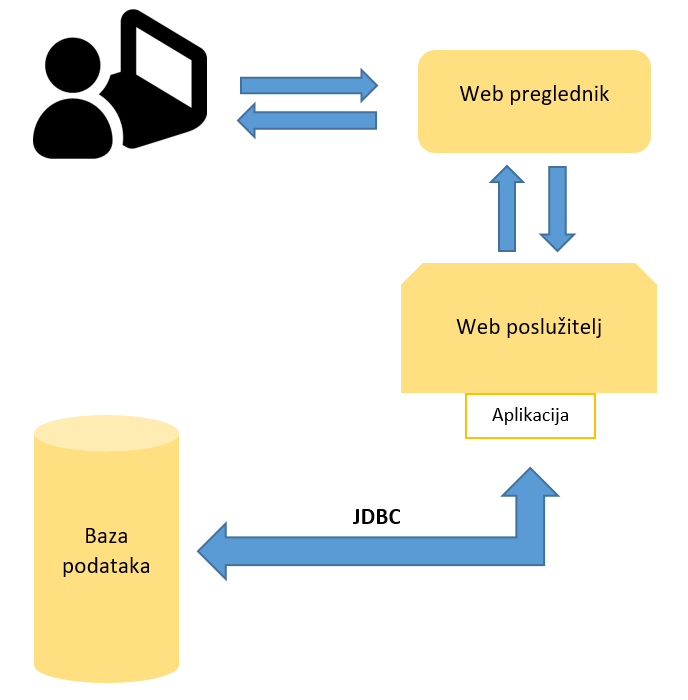
\includegraphics[scale=0.8]{arhitektura/arhitektura_sustava.png} %veličina slike u odnosu na originalnu datoteku i pozicija slike
					\centering
					\caption{Arhitektura sustava}
					\label{fig:arhitektura}
		\end{figure}

	\vspace{5mm} %5mm vertical space

		Web aplikacija će se temeljiti na modelu klijent-poslužitelj, što je danas i najčešće korišteni model. Korisnik šalje zahtjeve na koje odgovara poslužitelj, dok i jedna i druga strana mogu imati korisničku i poslužiteljsku aplikaciju.

	\vspace{10mm} %10mm vertical space

		\textbf{\underline{Web preglednik:} }\\

			Klijentski program, zvan preglednik, služi kao korisničko sučelje za pregledavanje sadržaja na Webu. On je taj koji šalje zahtjev Web poslužitelju i prikazuje primljene podatke u obliku Web stranica korisniku. Dakle, preglednik će primljene podatke u obliku koda interpretirati u nešto korisniku razumljivo, odnosno prikazat će korisničko sučelje naše aplikacije. Konačan prikaz aplikacije može uključivati više dohvata resursa i često može sadržavati dodatke te pomoćne aplikacije za prikaz formata koje izvorno ne podržava.

		\vspace{5mm} %5mm vertical space
		\textbf{\underline{Web poslužitelj:} }\\

		Poslužiteljski program poslužuje resurse smještene na poslužiteljskom računalu ili na drugim izvorima i odgovara na zahtjeve korisnika. Komunikacija se odvija preko HTTP/HTTPS (\textit{HyperText Transfer Protocol/Secure}) standardnog internetskog aplikacijskog protokola koji ima mogućnost prijenosa raznih vrsta podataka i proširiv je prema novim formatima podataka. Poslužitelj je zaslužan za pokretanje Web aplikacije.

		\vspace{5mm} %5mm vertical space
		
		\textbf{\underline{Web aplikacija:} }\\

		Za realizaciju frontend-a, odnosno korisničkog sučelja upotrijebit ćemo React kao bazu unutar kojega ćemo koristiti jezike HTML, TypeScript i CSS. TypeScript nam omogućava izradu dinamičkih web stranica u kombinaciji s HTML-om i CSS-om i njime možemo mijenjati sadržaj na stranici ovisno o načinu interakcije korisnika sa stranicom. Uz ove navedene tehnologije moguće je napraviti moderno korisničko sučelje jedne Web i mobilne aplikacije. Nakon što Web preglednik korisniku prikaže aplikaciju ''Planinarski dnevnik'', korisnik može izvršiti određenu naredbu odabirom neke od funkcionalnosti aplikacije. Hoće li pristupiti bazi podataka ovisi o samoj akciji. Za komunikaciju s bazom podataka koristi se JDBC koji predstavlja sučelje aplikacijskog programiranja za jezik Java i definira kako klijent može pristupiti bazi podataka. Pruža metode za upit i ažuriranje u bazi podataka te je orijentiran prema relacijskim bazama podataka. Što se tiče backend-a koristimo Spring Boot i MVC arhitekturu. 


		\vspace{5mm} %5mm vertical space

		\textbf{Spring Boot} pruža fleksibilan način konfiguriranja Java Beans, XML konfiguracija i transakcija baze podataka te bitno olakšava upravljanje ovisnostima. Svaka pokrenuta usluga ima svoj postupak, a time se postiže jednostavan model za podršku aplikacijama.  


		\vspace{5mm} %5mm vertical space

		\textbf{Model – View – Controller} je obrazac koji razdvaja aplikaciju u tri glavne logičke komponente: Model, View i Controller. Svaka od nabrojenih komponenti ima zadatak rukovati s određenim razvojnim aspektima aplikacije. Također, one su nezavisne jedna od druge i kao rezultat toga je jednostavno dodavanje i preoblikovanje svojstava.


		\vspace{5mm} %5mm vertical space

		\begin{itemize}
		\item \textbf{Model}	
		
		Poznat je kao najniža razina što znači da je odgovoran za održavanje podataka s kojima korisnik radi. Glavni zadatak je dohvat, manipulacija podatcima i uglavnom on surađuje s bazom podataka. Reagira na zahtjeve Controller-a jer on nikada sam ne razgovara s bazom podataka i nakon komunikacije prosljeđuje potrebne podatke Controllor-u. Jedna od bitnijih stvari za napomenuti je da Model nikada izravno ne komunicira s View.

		\item \textbf{View}
		
		Služi za prikazivanje podataka na način da zapravo generira korisničko sučelje za korisnika. Ti podaci su rezultat rada Model-a, ali se oni ne preuzimaju izravno već putem Controller-a tako da View surađuje samo s Controller-om. 

		\item \textbf{Controller}

		Djeluje u službi posrednika između komponenti Model i View. Ne mora brinuti o rukovanju logikom podataka, već samo govori Model-u što treba učiniti. Nakon primanja podataka od Model-a, on ih obrađuje i konačno rezultat prosljeđuje do View-a gdje objašnjava kako ih prikazati korisniku. Ako je došlo do promjena, Controller je zadužen za ažuriranje View-a.


		\end{itemize}


		\begin{figure}[H]
					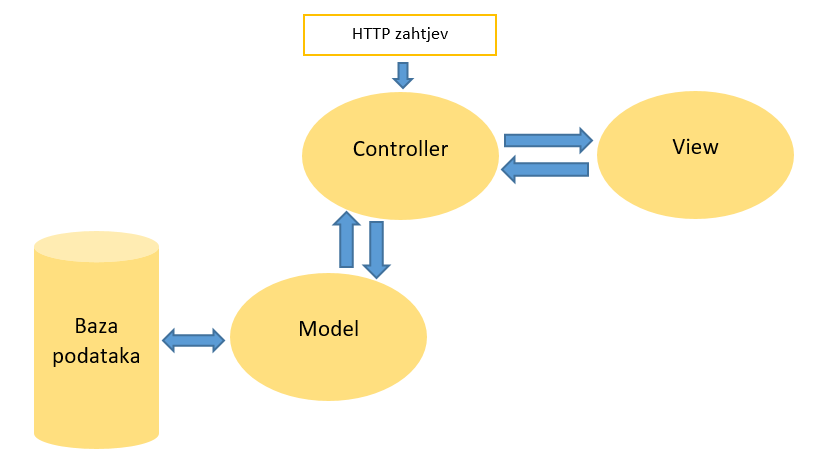
\includegraphics[scale=0.8]{arhitektura/mvc.png} %veličina slike u odnosu na originalnu datoteku i pozicija slike
					\centering
					\caption{Model - View - Controller}
					\label{fig:arhitektura}
		\end{figure}

		\section{Baza podataka}
			
		Za naš projekt odabrali smo \textbf{relacijsku bazu podataka} zbog njezine pogodnosti da prikaže mali dio stvarnog svijeta bez redundancije unutar same baze. Dohvaćanje podataka je relativno brzo i lagano se može paralelizirati. Specifičnu implementaciju relacijske baze podataka koju smo odabrali je \textbf{PostgreSQL}. To je baza podataka otvorenog koda s preko 30 godina aktivnog razvoja zbog kojeg je zaslužila svoju čvrstu reputaciju za pouzdanost, bogatstvo opcijama i visokim performansama. Zbog načina na koji je SQL standard napisan, vrlo je slična ostalim SQL bazama podataka.\\ 
		
		Tijekom razvoja koristimo \textbf{H2 bazu}. To je privremena baza podataka koja služi za testiranje koda. Svi zapisi u njoj se nalaze u privremenoj memoriji i nisu perzistentni. Zbog toga je odlična za testiranje. Ona je otvorenog koda, napisana u Javi i ima čvrste sigurnosne postavke. Na nju se možemo povezati s više konekcija i baza podataka je enkriptirana SHA-256 enkripcijom. Ima vrlo malu potrošnju memorije i zauzima relativno malo prostora na disku (oko 2MB). \\ 
		
		Također koristimo \textbf{JPA (Java Persistence API)} koje samo sadrži sučelja za stvaranje Persistence layouta. Dopušta nam da mapiramo entitete tablica i veze između tablica na objekte u Javi. Ovo sučelje definira svoj vlastiti jezik za upite (JPQL). JPQL prevoditelj interpretira kod i piše SQL upite. JPA ne možemo samostalno koristiti, već nam treba konkretna implementacija toga sučelja. Implementacija koju ćemo mi koristiti se zove Hibernate. \\ 
		
		Na bazu podataka se iz Jave spajamo preko \textbf{JdbcTemplatea}. To je snažni mehanizam za spajanje i izvođenje SQL upita. On nam smanjuje količinu koda koju moramo napisati kako bismo izvršavali upite, kao što je spajanje na bazu, kreiranje izraza i zatvaranje konekcija. \\
		\newpage
	Naš model baze podataka sastoji se od sljedećih \textbf{glavnih} i \underline{veznih} tablica:
		\begin{itemize}[noitemsep]
		\item \textbf{user}
\item \textbf{roles}
\item \textbf{mountain$\_$lodge}
\item \textbf{mountain$\_$path}
\item \textbf{event}
\item \textbf{hill}
\item \textbf{utility}
\item \textbf{badge}
\item \textbf{message}
\item \underline{friendships}
\item \underline{frienship$\_$request}
\item \underline{frienship$\_$notifications}
\item \underline{user$\_$badge}
\item \underline{mountain$\_$lodge$\_$utility}

\item \underline{event$\_$attendance}
\item \underline{mountain$\_$path$\_$report}
\item \underline{mountain$\_$path$\_$grade}
\item \underline{path$\_$user$\_$wishlist}
\item \underline{mountain$\_$path$\_$user$\_$archived}
\item
\underline{community$\_$event$\_$mountain$\_$path}
\item
\underline{mountain$\_$lodge$\_$user$\_$archived}

\end{itemize}
\newpage
\subsection{Opis tablica}
Primarni ključevi su označeni \textbf{podebljano}, dok su strani ključevi \underline{podvučeni}. \\
Prikazane su i sve vezne tablice, tako da se nad glavnim tablicama Many-To-Many veze neće navoditi.

%Tablice
\textbf{user} -  ovaj entitet sadrži sve važne informacije o korisniku aplikacije.
Sadrži atribute: "id", "name", "email", "password", "image",
"place$\_$of$\_$residence", "date$\_$of$\_$birth", "role$\_$id", "current$\_$user$\_$id" i "description" koji redom predstavljaju jedinstveni identifikacijski broj korisnika, ime i prezime, e-mail korisnika, lozinku korisnika, sliku vidljivu na profilu korisnika, mjesto stanovanja korisnika te datum rođenja korisnika, id role korisnika, id trenutnog korisnika i opis.
Neki podaci o korisniku, kao što su mjesto stanovanja i datum rođenja su opcionalni, i ako ih korisnik ne ispuni njihova vrijednost je \textit{NULL}. Atribut "role\_id" je strani ključ koji referencira entitet \textbf{roles} te se radi o Many-To-One vezi. 

\begin{longtabu} to \textwidth {|X[6, l]|X[6, l]|X[20, l]|}
\hline \multicolumn{3}{|c|}{\textbf{user - (Korisnik)}}	 \\[3pt] \hline
\endfirsthead

\hline \multicolumn{3}{|c|}{\textbf{user - (Korisnik)}}	 \\[3pt] \hline
\endhead

\hline 
\endlastfoot

\textbf{id} & BIGINT	&  	jedinstveni identifikacijski broj korisnika	\\ \hline
name	& VARCHAR &  ime i prezime korisnika 	\\ \hline 
email & VARCHAR &  e-mail pomoću kojeg se korisnik prijavljuje u sustav \\ \hline 
description	& VARCHAR &  opis korisnika, unos je opcionalan 	\\ \hline 
password & VARCHAR	&  	lozinka pomoću koje se korisnik prijavljuje u sustav	\\ \hline 
place\_of
\_residence & VARCHAR	&  	mjesto stanovanja korisnika, unos je opcionalan	\\ \hline 
image & BYTEA	&  	slika vidljiva na profilu korisnika	\\ \hline 
current\_user\_id & BIGINT	&  	id trenutnog korisnika	\\ \hline 
\underline{role\_id} & BIGINT & strani ključ role iz tablice \textbf{roles}\\ \hline
date\_of\_birth & DATE & datum rođenja korisnika, unos je opcionalan \\ \hline


\end{longtabu}
\vspace{10mm}

\textbf{roles} Ovaj entitet modelira ulogu korisnika unutar aplikacije, tzv. "aplikativne role". Određuje razinu ovlasti koje korisnik ima. Sadrži atribute: "id" i "name" koji predstavljaju jedinstveni identifikator uloge te naziv uloge. Dopuštene uloge u našoj aplikaciji su: Planinar, Dežurni planinar i Administrator.

\begin{longtabu} to \textwidth {|X[6, l]|X[6, l]|X[20, l]|}

\hline \multicolumn{3}{|c|}{\textbf{roles - (Uloga)}}	 \\[3pt] \hline
\endfirsthead

\hline \multicolumn{3}{|c|}{\textbf{role - ime tablice}}	 \\[3pt] \hline
\endhead

\hline 
\endlastfoot

\textbf{id} & BIGINT	&  jedinstveni ID uloge	\\ \hline
name	& VARCHAR &  ime uloge 	\\ \hline 

\end{longtabu}

\vspace{10mm}		

\textbf{mountain\_lodge} Ovaj entitet modelira jedan planinarski dom. Sadrži atribute: "id", "name", "image", "elevation" i "hill\_id" koji predstavljaju jedinstveni identifikator planinarskog doma, naziv planinarskog doma, sliku planinarskog doma, nadmorsku visinu te jedinstveni identifikator zemljopisnog područja (visočja) na kojemu se planinarski dom nalazi. Unos slike za neki planinarski dom je opcionalan, a ako se atribut ne popuni njegova vrijednost je \textit{NULL}. Atribut "hill\_id" predstavlja strani ključ koji referencira entitet \textbf{hill} te se radi o Many-To-One vezi. 

\begin{longtabu} to \textwidth {|X[6, l]|X[6, l]|X[20, l]|}

\hline \multicolumn{3}{|c|}{\textbf{mountain\_lodge - (Planinarski dom)}}	 \\[3pt] \hline
\endfirsthead

\hline \multicolumn{3}{|c|}{\textbf{mountain\_lodge - ime tablice}}	 \\[3pt] \hline
\endhead

\hline 
\endlastfoot

\textbf{id} & BIGINT	&  	jedinstveni identifikacijski broj planinarskog doma 	\\ \hline
name	& VARCHAR &   naziv planinarskog doma	\\ \hline 
image & BYTEA &  slika planinarskog doma koja se prikazuje unutar aplikacije, unos je opcionalan \\ \hline 
elevation & INTEGER & nadmorska visina na kojoj se planinarski dom nalazi izražena u kilometrima \\ \hline 
\underline{hill\_id} & BIGINT	&  strani ključ na tablicu \textbf{hill}, a predstavlja identifikator visočja na kojemu se nalazi planinarski dom	\\ \hline 


\end{longtabu}
\vspace{10mm}		


\textbf{utility} Ovaj entitet modelira značajke infrastrukture pojedinog doma. Sadrži atribute "id" i "name" koji predstavljaju jedinstveni identifikacijski broj značajke te naziv značajke. Primjeri takvih značajki su pitka voda, hrana, smještaj, internet.

\newpage
\begin{longtabu} to \textwidth {|X[6, l]|X[6, l]|X[20, l]|}

\hline \multicolumn{3}{|c|}{\textbf{utility - (Pogodnost, značajka)}}	 \\[3pt] \hline
\endfirsthead

\hline \multicolumn{3}{|c|}{\textbf{utility - ime tablice}}	 \\[3pt] \hline
\endhead

\hline 
\endlastfoot

\textbf{id} & BIGINT	&  jedinstveni identifikator značajke\\ \hline
name	& VARCHAR &  naziv značajke/pogodnosti \\ \hline 

\end{longtabu}
\vspace{10mm}		

\textbf{hill} Ovaj entitet modelira pojedino zemljopisno područje, odnosno visočje na kojemu se nalazi pojedini planinarski dom ili planinarska staza. Sadrži atribute: "id" i "name" koji predstavljaju jedinstveni identifikacijski broj visočja te naziv visočja.

\begin{longtabu} to \textwidth {|X[6, l]|X[6, l]|X[20, l]|}

\hline \multicolumn{3}{|c|}{\textbf{hill - (Visočje)}}	 \\[3pt] \hline
\endfirsthead

\hline \multicolumn{3}{|c|}{\textbf{hill - ime tablice}}	 \\[3pt] \hline
\endhead

\hline 
\endlastfoot

\textbf{id} & BIGINT	&  jedinstveni ID visočja 	\\ \hline
name & VARCHAR	&  ime visočja 	\\ \hline


\end{longtabu}
\vspace{10mm}

\textbf{mountain\_path} Ovaj entitet sadrži informacije o pojedinoj planinarskoj stazi. Sadrži atribute: "id", "name", "start\_point", "end\_point", "avg\_walk\_time", "length", "sea\_level\_diff", "date\_created", "is\_private", "author\_id" i "hill\_id" koji redom predstavljaju jedinstveni identifikacijski broj planinarske staze, naziv staze, polazišnu točku, završnu toku, prosječno vrijeme potrebno da se prepješači staza, duljinu staze, razliku u nadmorskoj visini između početne i završne točke, datum kreiranja pojedine staze od strane korisnika unutar naše aplikacije, vrijednost koja govori je li staza privatna ili javna, korisnika koji je stvorio stazu te identifikator visočja na kojemu se staza nalazi. Atribut "author\_id" te atribut "hill\_id" su strani ključevi obzirom na tablicu \textbf{user} odnosno \textbf{hill} te se radi o Many-To-One vezama.

\begin{longtabu} to \textwidth {|X[6, l]|X[6, l]|X[20, l]|}

\hline \multicolumn{3}{|c|}{\textbf{mountain\_path - (Planinarska staza)}}	 \\[3pt] \hline
\endfirsthead

\hline \multicolumn{3}{|c|}{\textbf{mountain\_path - (Planinarska staza)}}	 \\[3pt] \hline
\endhead

\hline 
\endlastfoot

\textbf{id} & BIGINT	& jedinstveni identifikacijski broj planinarske staze	\\ \hline
name	& VARCHAR &  naziv staze	\\ \hline 
start\_point & VARCHAR & naziv početne točke staze  \\ \hline 
end\_point & VARCHAR &  naziv završne točke staze \\ \hline 
avg\_walk\_time & TIME &  prosječno vrijeme potrebno za prepješačiti stazu\\ \hline 
length & INTEGER & duljina staze u metrima\\ \hline 
sea\_level\_diff & INTEGER & razlika u nadmorskoj visini između početne i završne točke staze\\ \hline 
date\_created & DATE &  datum stvaranja staze unutar aplikacije\\ \hline 
is\_private & BOOLEAN	&  atribut koji govori je li korisnik stazu stvara privatno ili javno  \\ \hline 
\underline{author\_id} & BIGINT	&  	identifikacijski broj korisnika koji je stvorio stazu unutar aplikacije\\ \hline 
\underline{hill\_id} & BIGINT	&  identifikacijski broj visočja na kojemu se staza nalazi\\ \hline 


\end{longtabu}
\vspace{10mm}

\textbf{event} Ovaj entitet modelira jedan događaj koji stvara korisnik unutar naše aplikacije. Jedan događaj počinje u određeno vrijeme "start\_date", te završava u određeno vrijeme: "end\_date". Svaki događaj, odnosno planinarski izlet sastoji se od jedne ili više planinarskih staza koje se obilaze tijekom tog planinarskog izleta. Osim toga, planinarski izlet ima svoj opis: "description", gdje korisnik može reći više pojedinosti o samom planinarskom izletu. Osim toga, ovaj entitet sadrži atribute: "event\_id", "name", "date\_created" i "author\_id" koji predstavljaju jedinstveni identifikacijski broj događaja, naziv događaja, vrijeme kada je korisnik stvorio događaj unutar aplikacije te jedinstveni identifikacijski broj korisnika koji je stvorio događaj. Atribut "user\_id" je strani ključ koji se odnosi na tablicu \textbf{user} te se radi o Many-To-One vezi.

\begin{longtabu} to \textwidth {|X[6, l]|X[6, l]|X[20, l]|}

\hline \multicolumn{3}{|c|}{\textbf{event - (Planinarski događaj)}}	 \\[3pt] \hline
\endfirsthead

\hline \multicolumn{3}{|c|}{\textbf{event - (Planinarski događaj)}}	 \\[3pt] \hline
\endhead

\hline 
\endlastfoot

\textbf{event\_id} & BIGINT	&  	jedinstveni identifikacijski broj planinarskog izleta 	\\ \hline
name	& VARCHAR & naziv događaja 	\\ \hline 
description & VARCHAR &  pojedinosti vezane uz događaj \\ \hline 
start\_date & TIMESTAMP	&  vrijeme i datum početka planinarskog izleta	\\ \hline 
end\_date & TIMESTAMP	&  	vrijeme i datum završetka planinarskog izleta	\\ \hline 
date\_created & TIMESTAMP	&  vrijeme i datum stvaranja izleta unutar aplikacije\\ \hline 
\underline{user\_id} & BIGINT	& jedinstveni identifikacijski broj korisnika koji je stvorio događaj unutar aplikacije		\\ \hline 


\end{longtabu}
\vspace{10mm}

\textbf{badge} Ovaj entitet modelira jedan bedž, odnosno priznanje koje korisnik može zaslužiti kao planinar. Korisnik priznanja zaslužuje za svoju aktivnost koja se gleda na osnovu arhive planinarskih domova i staza, te se uzimaju u obzir značajke kao što su: broj posjećenih planinarskih domova, broj odrađenih planinarskih staza i sl. Entitet sadrži atribute "id", "name" i "description" koji predstavljaju jedinstveni identifikacijski broj priznanja, naziv priznanja te opis priznanja.

\begin{longtabu} to \textwidth {|X[6, l]|X[6, l]|X[20, l]|}

\hline \multicolumn{3}{|c|}{\textbf{badge - (Priznanje)}}	 \\[3pt] \hline
\endfirsthead

\hline \multicolumn{3}{|c|}{\textbf{badge - (Priznanje)}}	 \\[3pt] \hline
\endhead

\hline 
\endlastfoot

\textbf{id}	& BIGINT &   jedinstveni identifikacijski broj priznanja	\\ \hline 
name & VARCHAR &  naziv priznanja \\ \hline 
description & VARCHAR &  opis priznanja \\ \hline 


\end{longtabu}

\vspace{10mm}

\textbf{message} Ovaj entitet modelira poruke koje korisnik može slati administratoru u slučaju npr. otvaranja novog planinarskog doma. Sadrži atribute: "id", "status", "error", "message\_name", "message\_content" i "user\_id" koji redom predstavljaju jedinstveni identifikacijski broj poruke, status poruke, mjesto gdje je prijavljena greška, naslov poruke, sadržaj poruke i id korisnika koji je poslao poruku.

\begin{longtabu} to \textwidth {|X[6, l]|X[6, l]|X[20, l]|}

\hline \multicolumn{3}{|c|}{\textbf{message - (Poruke administratoru)}}	 \\[3pt] \hline
\endfirsthead

\hline \multicolumn{3}{|c|}{\textbf{badge - (Priznanje)}}	 \\[3pt] \hline
\endhead

\hline 
\endlastfoot

\textbf{id}	& BIGINT &   jedinstveni identifikacijski broj poruke	\\ \hline 
status & VARCHAR &  status poruke \\ \hline 
error & VARCHAR &  mjesto gdje je nastala pogrška \\ \hline 
message\_name & VARCHAR &  naslov poruke \\ \hline 
message\_content & VARCHAR &  sadržaj poruke \\ \hline 
\underline{user\_id} & BIGINT	& jedinstveni identifikacijski broj korisnika koji je stvorio poruku unutar aplikacije		\\ \hline 

\end{longtabu}
\vspace{10mm}


\textbf{friendships} Ovo je vezna tablica koja sadrži Many-To-Many vezu između dva korisnika, a služi nam za modeliranje prijateljstava, odnosno pripadanja istoj planinarskoj zajednici. Sadrži atribute "current\_user\_id" i "friend\_id" koji predstavljaju strane ključeve na tablicu \textbf{user} i govore nam tko su korisnici koji pripadaju istoj zajednici.

\begin{longtabu} to \textwidth {|X[6, l]|X[6, l]|X[20, l]|}

\hline \multicolumn{3}{|c|}{\textbf{friendships - (Prijatelji)}}	 \\[3pt] \hline
\endfirsthead

\hline \multicolumn{3}{|c|}{\textbf{friendships - (Prijatelji)}}	 \\[3pt] \hline
\endhead

\hline 
\endlastfoot

\underline{current\_user\_id} & BIGINT	&  strani ključ koji se odnosi na jednog korisnika člana veze "prijatelji"	\\ \hline
\underline{friend\_id}	& BIGINT &   strani ključ koji se odnosi na drugog korisnika člana veze "prijatelji"\\ \hline 
%\cellcolor{LightBlue} primjer	& VARCHAR &   	\\ \hline 


\end{longtabu}
\vspace{10mm}

\textbf{friendship\_request} Ovaj entitet sadrži informaciju o poslanom zahtjevu za prijateljstvo između 2 korisnika. Sadrži atribute: "sender" te "reciever" koji su oba strani ključevi iz tablice \textbf{user}, a predstavljaju identifikacijski broj pošiljatelja te primatelja zahtjeva za prijateljstvo. Radi se o refleksivnoj Many-to-Many vezi.

\begin{longtabu} to \textwidth {|X[6, l]|X[6, l]|X[20, l]|}

\hline \multicolumn{3}{|c|}{\textbf{friendship\_request - (Zahtjevi za prijateljstvom)}}	 \\[3pt] \hline
\endfirsthead

\hline \multicolumn{3}{|c|}{\textbf{friendship\_req - (Zahtjevi za prijateljstvom)}}	 \\[3pt] \hline
\endhead

\hline 
\endlastfoot

\underline{sender} 
& BIGINT	&  strani ključ korisnika koji šalje zahtjev za prijateljstvom iz tablice \textbf{user} 	\\ \hline
\underline{recevier} 
& BIGINT &   strani ključ korisnika koji prima zahtjev za prijateljstvom	iz tablice \textbf{user}\\ \hline 
%\cellcolor{LightBlue} primjer	& VARCHAR &   	\\ \hline 


\end{longtabu}
\vspace{10mm}
\textbf{friendships\_notifications} Ovaj entitet sadrži informaciju o Many-To-Many odnosu između dva korisnika, a služi za modeliranje obavijesti korisnicima o prihvaćenim zahtjevima za prijateljstvo. Sadrži atribute "friendships\_notifications\_sender\_id" i "friendships\_notifications\_recevier\_id" koji predstvljaju strane ključeve na tablicu user i govore koji je korisnik kojem poslao zahtjev za prijateljstvo.

\begin{longtabu} to \textwidth {|X[6, l]|X[6, l]|X[20, l]|}

\hline \multicolumn{3}{|c|}{\textbf{friendships\_notifications}}	 \\[3pt] \hline
\endfirsthead

\hline \multicolumn{3}{|c|}{\textbf{friendships\_notifications}}	 \\[3pt] \hline
\endhead

\hline 
\endlastfoot

\underline{sender\_id} & BIGINT	& strani ključ 	korisnika  koji je poslao zahtjev iz tablice \textbf{user}	\\ \hline
\underline{recevier\_id} & BIGINT &   strani ključ korisnika koji je primio zahtjev iz tablice \textbf{user} \\ \hline


\end{longtabu}
\vspace{10mm}

\textbf{user\_badge} Ovaj entitet sadrži informaciju o Many-To-Many odnosu između bedževa (priznanja) i korisnika. Sadrži atribute: "user\_id", "badge\_id" i "date\_recieved" koji redom predstavljaju identifikacijski broj korisnika, identifikacijski broj priznanja te vrijeme dobivanja priznanja.

\begin{longtabu} to \textwidth {|X[6, l]|X[6, l]|X[20, l]|}

\hline \multicolumn{3}{|c|}{\textbf{user\_badge}}	 \\[3pt] \hline
\endfirsthead

\hline \multicolumn{3}{|c|}{\textbf{user\_badge}}	 \\[3pt] \hline
\endhead

\hline 
\endlastfoot

\underline{user\_id} & BIGINT	&  strani ključ korisnika kojem je pripisan pojedini bedž iz tablice \textbf{user}\\ \hline
\underline{badge\_id}	& BIGINT &  strani ključ bedža kojeg je dobio pojedini korisnik iz tablice \textbf{badge}	\\ \hline 
date\_recieved & DATE & datum dobivanja pojedinog bedža za određenog korisnika  \\ \hline 


\end{longtabu}
\vspace{10mm}

\textbf{event\_attendance} Modelira Many-To-Many vezu između korisnika i događaja (planinarskog izleta) na kojemu korisnik želi sudjelovati. Sadrži atribute "user\_id" te "event\_id" koji predstavljaju jedinstveni identifikator korisnika koji sudjeluje na događaju te jedinstveni identifikator događaja.

\begin{longtabu} to \textwidth {|X[6, l]|X[6, l]|X[20, l]|}

\hline \multicolumn{3}{|c|}{\textbf{event\_attendance}}	 \\[3pt] \hline
\endfirsthead

\hline \multicolumn{3}{|c|}{\textbf{event\_attendance}}	 \\[3pt] \hline
\endhead

\hline 
\endlastfoot

\underline{user\_id} & BIGINT	&  	strani ključ korisnika koji će prisustvovati događaju iz tablice \textbf{user}	\\ \hline
\underline{event\_id}	& BIGINT &  strani ključ događaja kojemu određena osoba pristupa iz tablice \textbf{event}\\ \hline 


\end{longtabu}
\vspace{10mm}		

\textbf{community\_event\_mountain\_path} Ovaj entitet sadrži informaciju o Many-To-Many vezi između planinarske staze i nekog planinarskog događaja. Sadrži atribute: "path\_id", "event\_id", "id" i "date\_traveled" koji predstavljaju identifikacijski broj planinarske staze, identifikacijski broj nekog planinarskog događaja, identifikacijski broj tablice. Osim toga, sadrži atribut "date\_traveled" koji nam govori o rednom broju dana tijekom kojeg se na određenom planinarskom događaju odrađuje određena planinarska staza.

\begin{longtabu} to \textwidth {|X[6, l]|X[6, l]|X[20, l]|}

\hline \multicolumn{3}{|c|}{\textbf{event\_path}}	 \\[3pt] \hline
\endfirsthead

\hline \multicolumn{3}{|c|}{\textbf{event\_path}}	 \\[3pt] \hline
\endhead

\hline 
\endlastfoot

{id} & BIGINT & jedinstveni identifikacijski broj\\ \hline
\underline{path\_id} & BIGINT	&  	strani ključ staze koja je dio nekog događaja iz tablice \textbf{mountain\_path}	\\ \hline
\underline{event\_id}	& BIGINT &  strani ključ događaja u kojem se pojedina staza odrađuje, iz tablice \textbf{event}	\\ \hline 
date\_traveled	& INTEGER &  redni broj dana koliko se unutar jednog događaja obilazi određena staza	\\ \hline 

\end{longtabu}
\vspace{10mm}

\textbf{mountain\_lodge\_utility} Vezna tablica koja modelira Many-to-Many vezu između planinarskih domova i infrastrukturnih značajki koje ti domovi posjeduju. Sadrži atribute "lodge\_id" te "utility\_id" koji predstavljaju identifikator planinarskog doma te identifikator odgovarajuće značajke.

\begin{longtabu} to \textwidth {|X[6, l]|X[6, l]|X[20, l]|}

\hline \multicolumn{3}{|c|}{\textbf{mountain\_lodge\_utility}}	 \\[3pt] \hline
\endfirsthead

\hline \multicolumn{3}{|c|}{\textbf{mountain\_lodge\_utility}}	 \\[3pt] \hline
\endhead

\hline 
\endlastfoot

\underline{lodge\_id} & BIGINT	&  strani ključ kojem je pripisan pojedini planinarski dom iz tablice  \textbf{mountain\_lodge}\\ \hline
\underline{utility\_id}	& BIGINT &  strani ključ kojem je pripisana pojedina značajka iz tablice \textbf{utility} \\ \hline 


\end{longtabu}
\vspace{10mm}

\textbf{mountain\_path\_grade} Vezna tablica koja nam govori o ocjenama koje pojedini korisnik dodijeljuje pojedinoj planinarskoj stazi. Radi se o Many-To-Many veznoj tablici. Sadrži atribute "user\_id", "path\_id" te "grade", koji redom predstavljaju identifikacijski broj korisnika, identifikacijski broj planinarske staze te ocjenu koju je taj korisnik dodijelio toj stazi.

\begin{longtabu} to \textwidth {|X[6, l]|X[6, l]|X[20, l]|}

\hline \multicolumn{3}{|c|}{\textbf{mountain\_path\_grade}}	 \\[3pt] \hline
\endfirsthead

\hline \multicolumn{3}{|c|}{\textbf{mountain\_path\_grade}}	 \\[3pt] \hline
\endhead

\hline 
\endlastfoot

\underline{user\_id} & BIGINT	& strani ključ korisnika koji daje ocjenu iz tablice \textbf{user}  	\\ \hline
\underline{path\_id}	& BIGINT &   strani ključ planinarske staze koja se ocjenjuje iz tablice \textbf{mountain\_path}	\\ \hline 
grade & INTEGER & ocjenu koju je korisnik dodijelio za konkretnu stazu  \\ \hline 


\end{longtabu}
\vspace{10mm}		

\textbf{path\_user\_wishlist} Vezna tablica koja modelira željene planinarske staze za pojedinog korisnika. To su staze koje korisnik ima namjeru prepješačiti, ali još nije uspio. Sadrži atribute "user\_id" i "path\_id" koji predstavljaju identifikator korisnika te identifikator staze koju korisnik želi prepješačiti.

\begin{longtabu} to \textwidth {|X[6, l]|X[6, l]|X[20, l]|}

\hline \multicolumn{3}{|c|}{\textbf{path\_user\_wishlist}}	 \\[3pt] \hline
\endfirsthead

\hline \multicolumn{3}{|c|}{\textbf{path\_user\_wishlist}}	 \\[3pt] \hline
\endhead

\hline 
\endlastfoot

\underline{user\_id} & BIGINT	& strani ključ korisnika  koji želi prepješačiti neku stazu iz tablice \textbf{user}	\\ \hline
\underline{path\_id} & BIGINT	& strani ključ staze koju korisnik želi prepješačiti iz tablice \textbf{mountain\_path}	\\ \hline


\end{longtabu}
\vspace{10mm}			

\textbf{mountain\_path\_user\_archived} Ovaj entitet sadrži informaciju o Many-To-Many odnosu između pojedinog korisnika i staza koje je već prepješačio, odnosno ovaj entitet modelira arhivu staza.

\begin{longtabu} to \textwidth {|X[6, l]|X[6, l]|X[20, l]|}

\hline \multicolumn{3}{|c|}{\textbf{mountain\_path\_user\_archived}}	 \\[3pt] \hline
\endfirsthead

\hline \multicolumn{3}{|c|}{\textbf{mountain\_path\_user\_archived}}	 \\[3pt] \hline
\endhead

\hline 
\endlastfoot

\underline{user\_id} & BIGINT	& strani ključ korisnika  koji je prepješačio pojedinu stazu iz tablice \textbf{user}	\\ \hline
path\_id	& BIGINT &   strani ključ staze koju je konkretni korisnik prepješačio iz tablice \textbf{mountain\_path}	\\ \hline 
date\_archived & DATE & datum kojeg je određeni korisnik prepješačio određenu stazu  \\ \hline 


\end{longtabu}
\vspace{10mm}
\textbf{mountain\_lodge\_user\_archived} Ovaj entitet sadrži informaciju o Many-To-Many odnosu između pojedinog korisnika i domova koje je već posjetio, odnosno ovaj entitet modelira arhivu planinarskih domova.

\begin{longtabu} to \textwidth {|X[6, l]|X[6, l]|X[20, l]|}

\hline \multicolumn{3}{|c|}{\textbf{mountain\_lodge\_user\_archived}}	 \\[3pt] \hline
\endfirsthead

\hline \multicolumn{3}{|c|}{\textbf{mountain\_lodge\_user\_archived}}	 \\[3pt] \hline
\endhead

\hline 
\endlastfoot

\underline{user\_id} & BIGINT	& strani ključ korisnika  koji je prepješačio pojedinu stazu iz tablice \textbf{user}	\\ \hline
mountain
\_lodge\_id	& BIGINT &   strani ključ doma kojeg je konkretni korisnik posjetio iz tablice \textbf{mountain\_lodge}	\\ \hline 
date\_archived & DATE & datum kojeg je određeni korisnik prepješačio određenu stazu  \\ \hline 


\end{longtabu}
\vspace{10mm}



			\subsection{Dijagram baze podataka}
				
				\begin{figure}[H]
					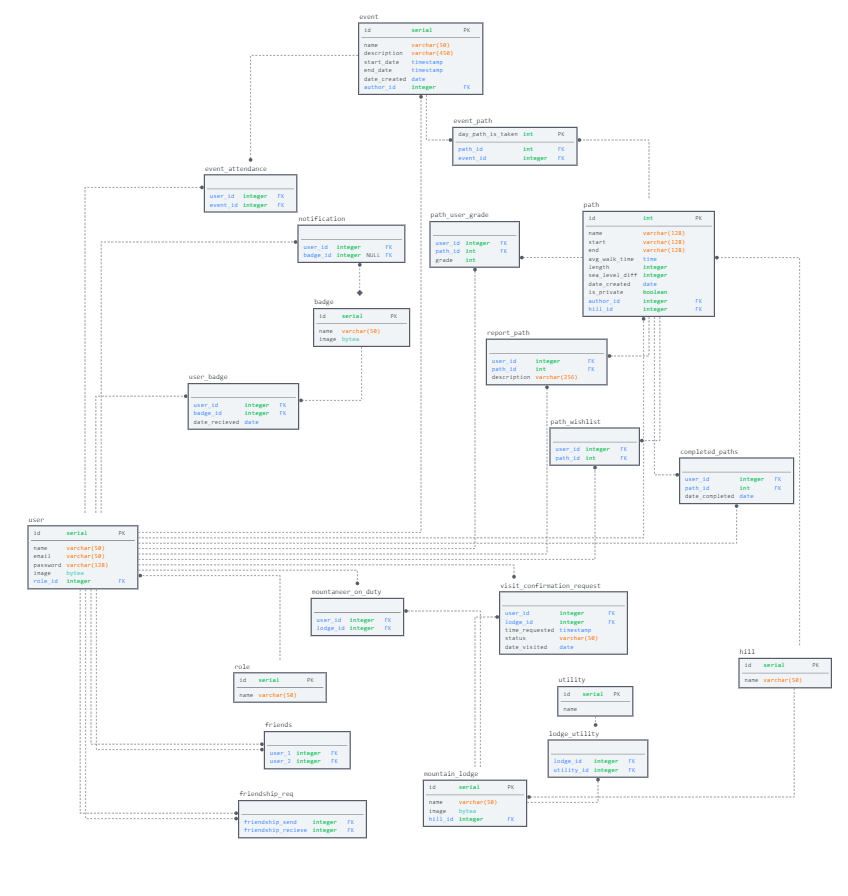
\includegraphics[scale=0.4, height=180mm]{slike/database.png} %veličina slike u odnosu na originalnu datoteku i pozicija slike
					\centering
					\caption{Dijagram baze podataka}
					\label{fig:dijagrambp}
				\end{figure}
			
			\eject
			
			
		\section{Dijagram razreda}
		
			\subsection{Konceptualni model dijagrama razreda}
			Prvi prikazani dijagram je konceptualni model dijagrama razreda. Na njemu su idejno prikazani razredi, njihove funkcionalnosti te odnosi između razreda. Svi razredi napravljeni su obzirom na obrasce uporabe i opise funkcionalnih zahtjeva.
		
			\begin{figure}[H]
				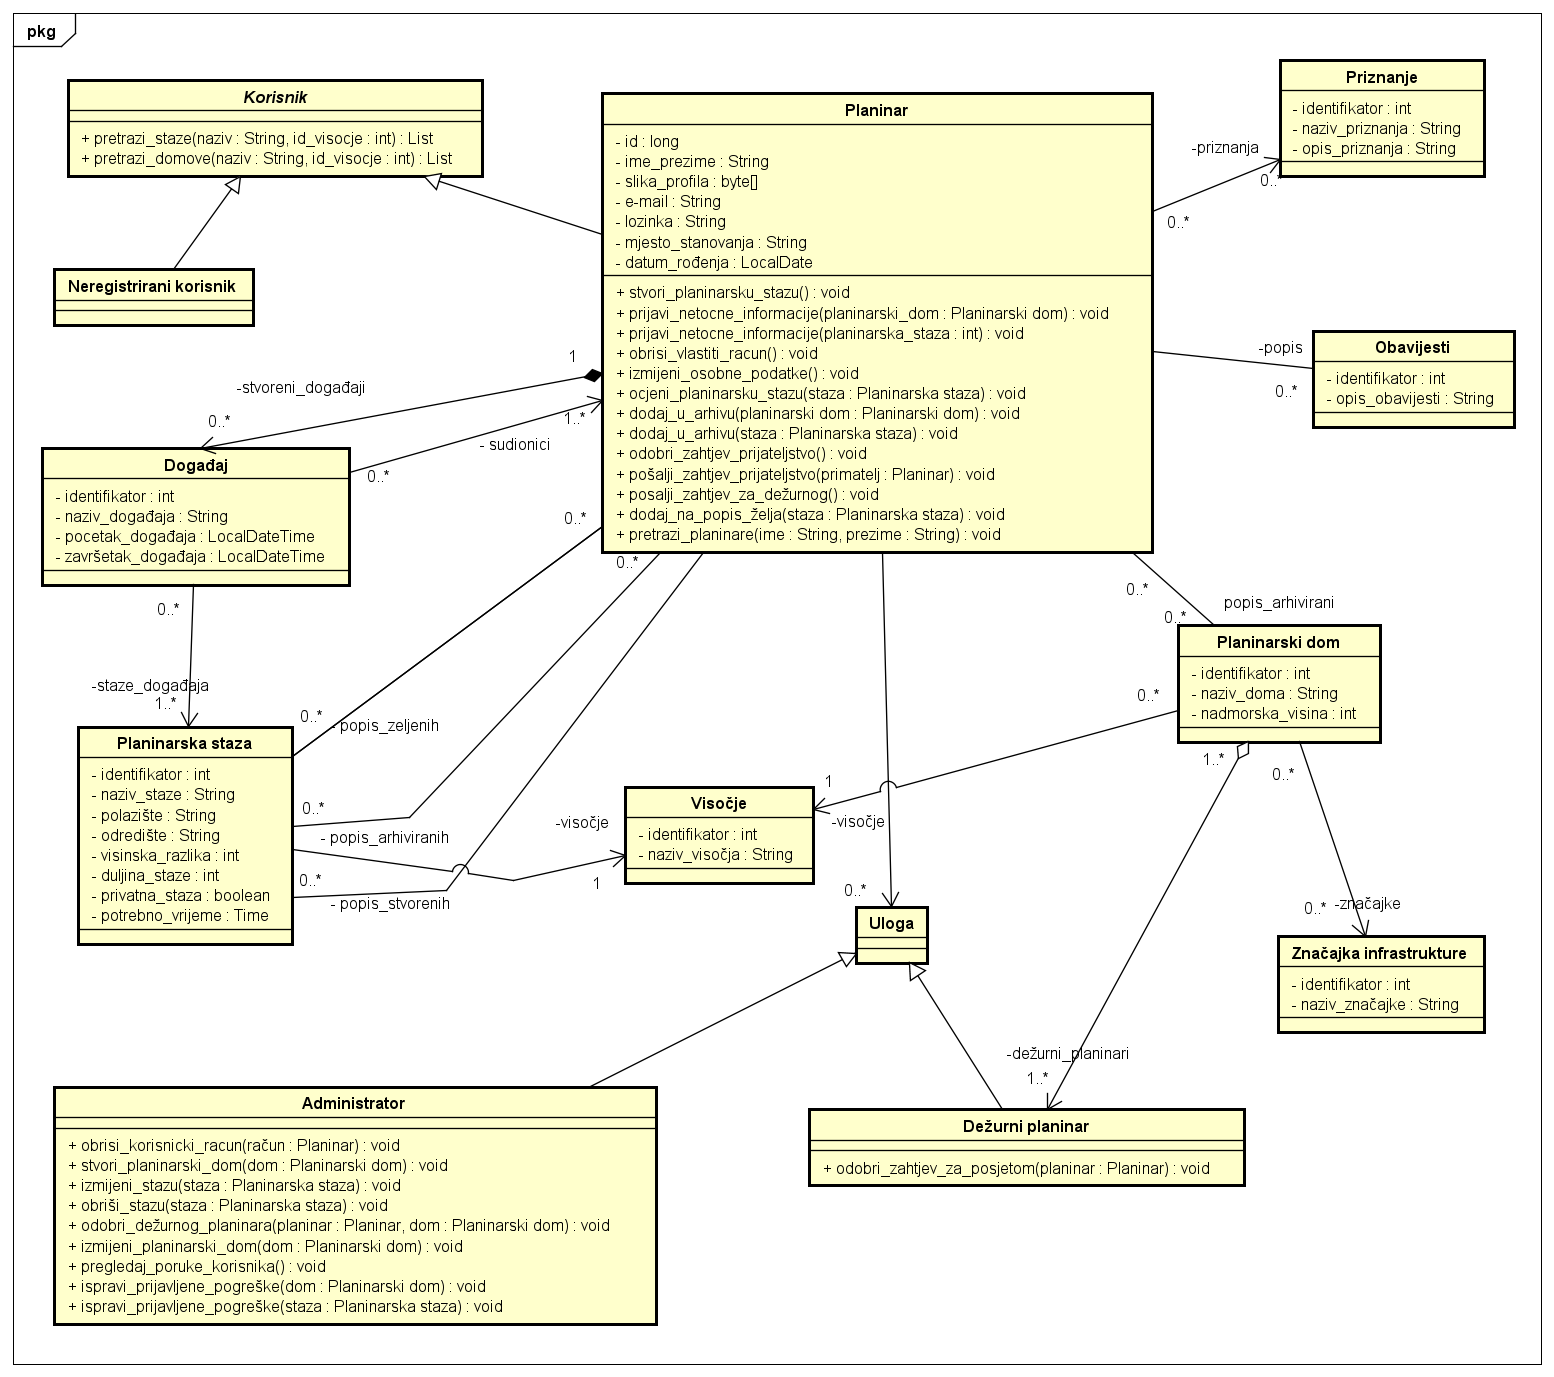
\includegraphics[scale=0.4, height=170mm, width=165mm]{dijagrami/domena-konceptualni.png} %veličina slike u odnosu na originalnu datoteku i pozicija slike
				\centering
				\caption{Dijagram razreda - konceptualni model}
				\label{fig:dijagrami_razreda3}
			\end{figure}
			
			\eject
			
			\subsection{Implementacijski dijagrami razreda - model sustava}
			\subsubsection{Sloj modela}
			Na dijagramima razreda nismo navodili podrazumijevane metode, gettere, settere te konstruktore.
			Na prva dva implementacijska dijagrama razreda prikazan je sloj modela. Temeljni razred je razred \textit{User}, za koji vidimo da ima najviše asocijacija s drugim razredima kao i nekoliko refleksivnih veza. Refleksivne veze redom čine članske varijable \textit{participatedEvents, friends, friendRequestNotifications, friendRequests}, a one predstavljaju događaje na kojima korisnik sudjeluje, popis prijatelja, popis obavijesti o prihvaćenim/odbijenim zahtjevima za prijateljstvo kao i popis zahtjeva za prijateljstvo. Osim toga, na prvom dijagramu \textit{User} je povezan i s razredom \textit{MountainPathGrade}, a ta veza predstavlja popis ocjena koje je korisnik dodijelio pojedinoj planinarskoj stazi, te je povezan s razredom \textit{MountainPath}, a ta veza predstavlja popis planinarskih staza koje je korisnik dodao u svoje favorite. Razred \textit{Role} predstavlja ulogu koju korisnik ima ako je registriran unutar aplikacije, a može biti \textbf{Admin} ili \textbf{Planinar}. Razred \textit{Badge} predstavlja priznanja koje korisnik može dobiti, a razredom \textit{UserBadge} povezan je s korisnikom. Razred \textit{MountainLodge} predstavlja planinarski dom. Razred \textit{MountainLodgeUserArchive} predstavlja vezu između korisnika i njegovih posjećenih planinarskih domova. Na isti način razred \textit{MountainPathUserArchive} predstavlja vezu između korisnika i njegovih prepješačenih planinarskih staza. Razredi \textit{FriendshipRequest} te \textit{Friendship} vezani su za obavijesti o zahtjevima za prijateljstvo te same veze prijateljstva između dva korisnika. Razred \textit{Utility} predstavlja infrastrukturne pogodnosti koje pruža pojedini planinarski dom, dok razred \textit{Hill} predstavlja visočje na kojemu se nalazi planinarski dom ili planinarska staza. Razred \textit{Message} predstavlja poruke/pogreške koje planinari šalju administratoru sustava. Naposljetku razred \textit{CommunityEvent} predstavlja neki planinarski događaj, a kao člansku varijablu ima \textit{participants} koja predstavlja korisnike koji su se prijavili za sudjelovanje. Planinarski događaj je preko razreda \textit{CommunityEventMountainPath} povezan s planinarskim stazama koje se obilaze unutar tog planinarskog događaja.
			
			\begin{figure}[H]
				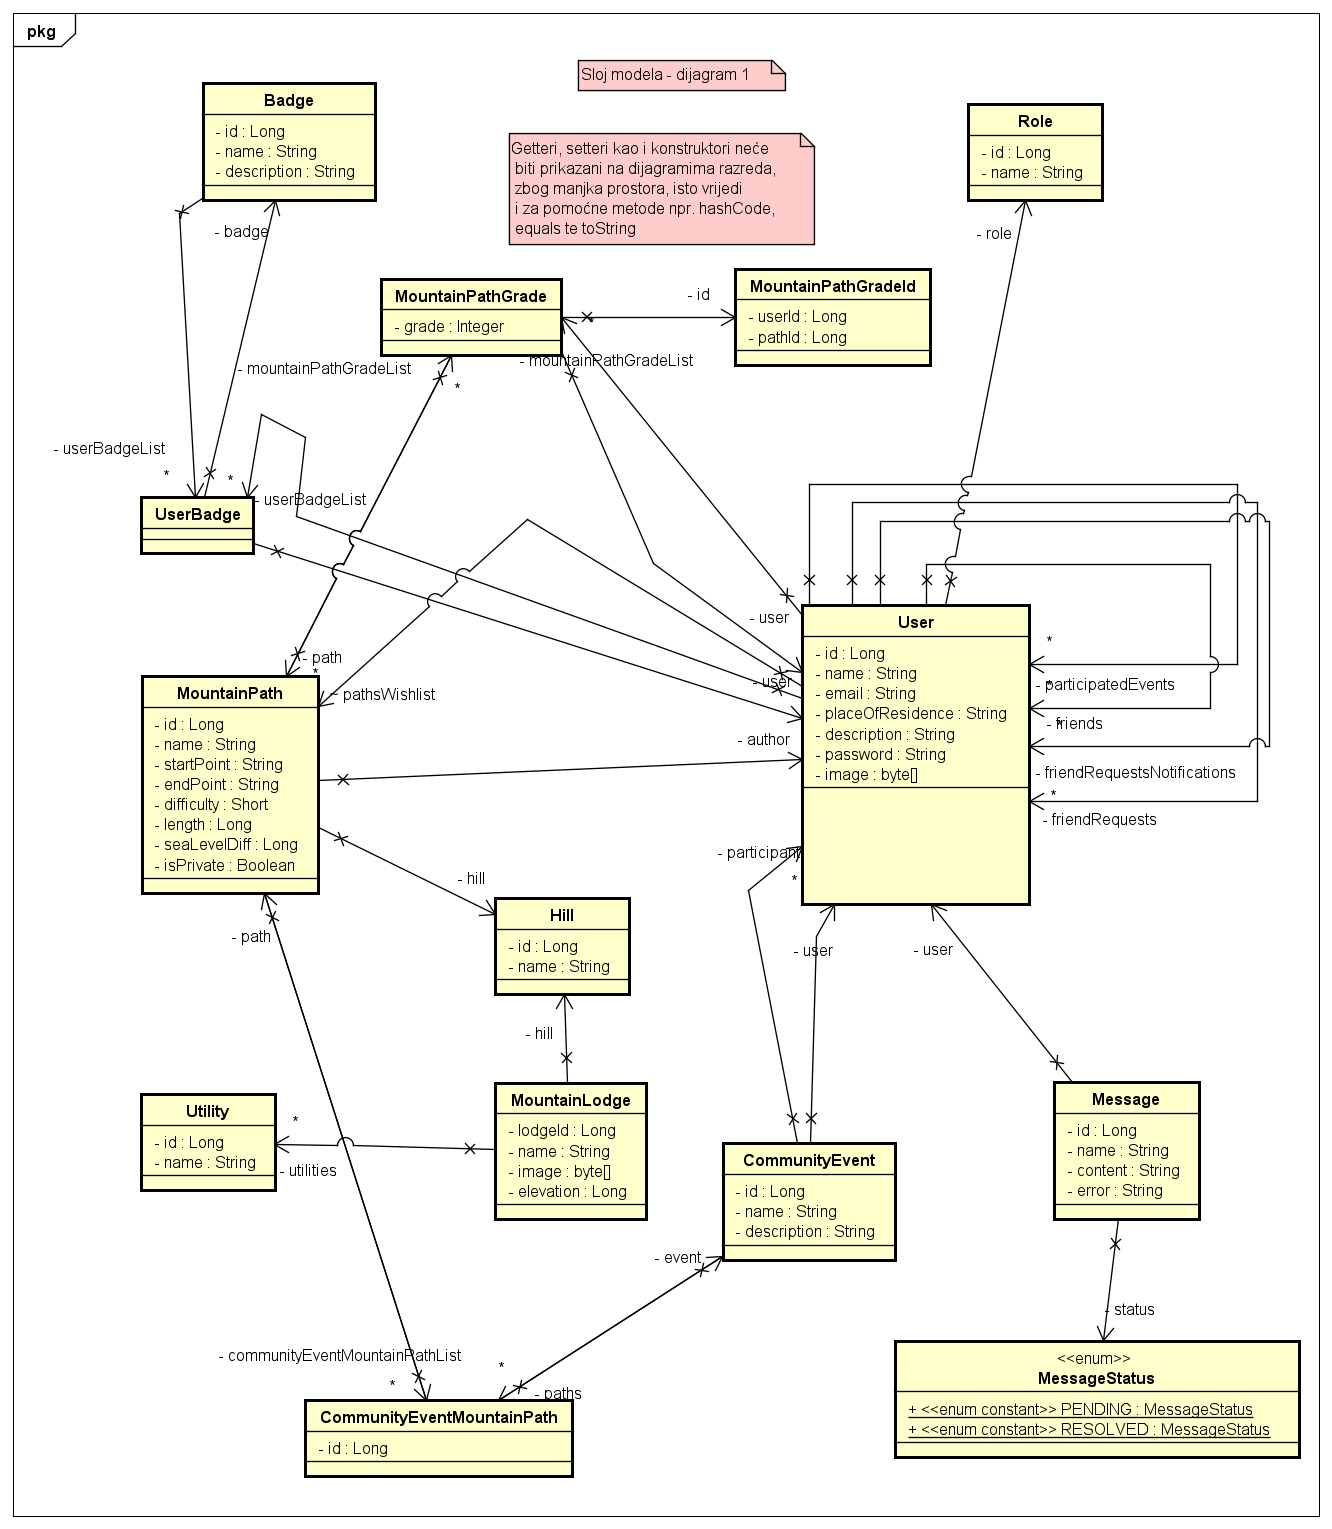
\includegraphics[scale=0.6, height=200mm, width=165mm]{dijagrami/model-dijagram1} %veličina slike u odnosu na originalnu datoteku i pozicija slike
				\centering
				\caption{Dijagram razreda - sloj modela prvi dijagram}
				\label{fig:dijagrami_razreda2}
			\end{figure}
		\begin{figure}[H]
			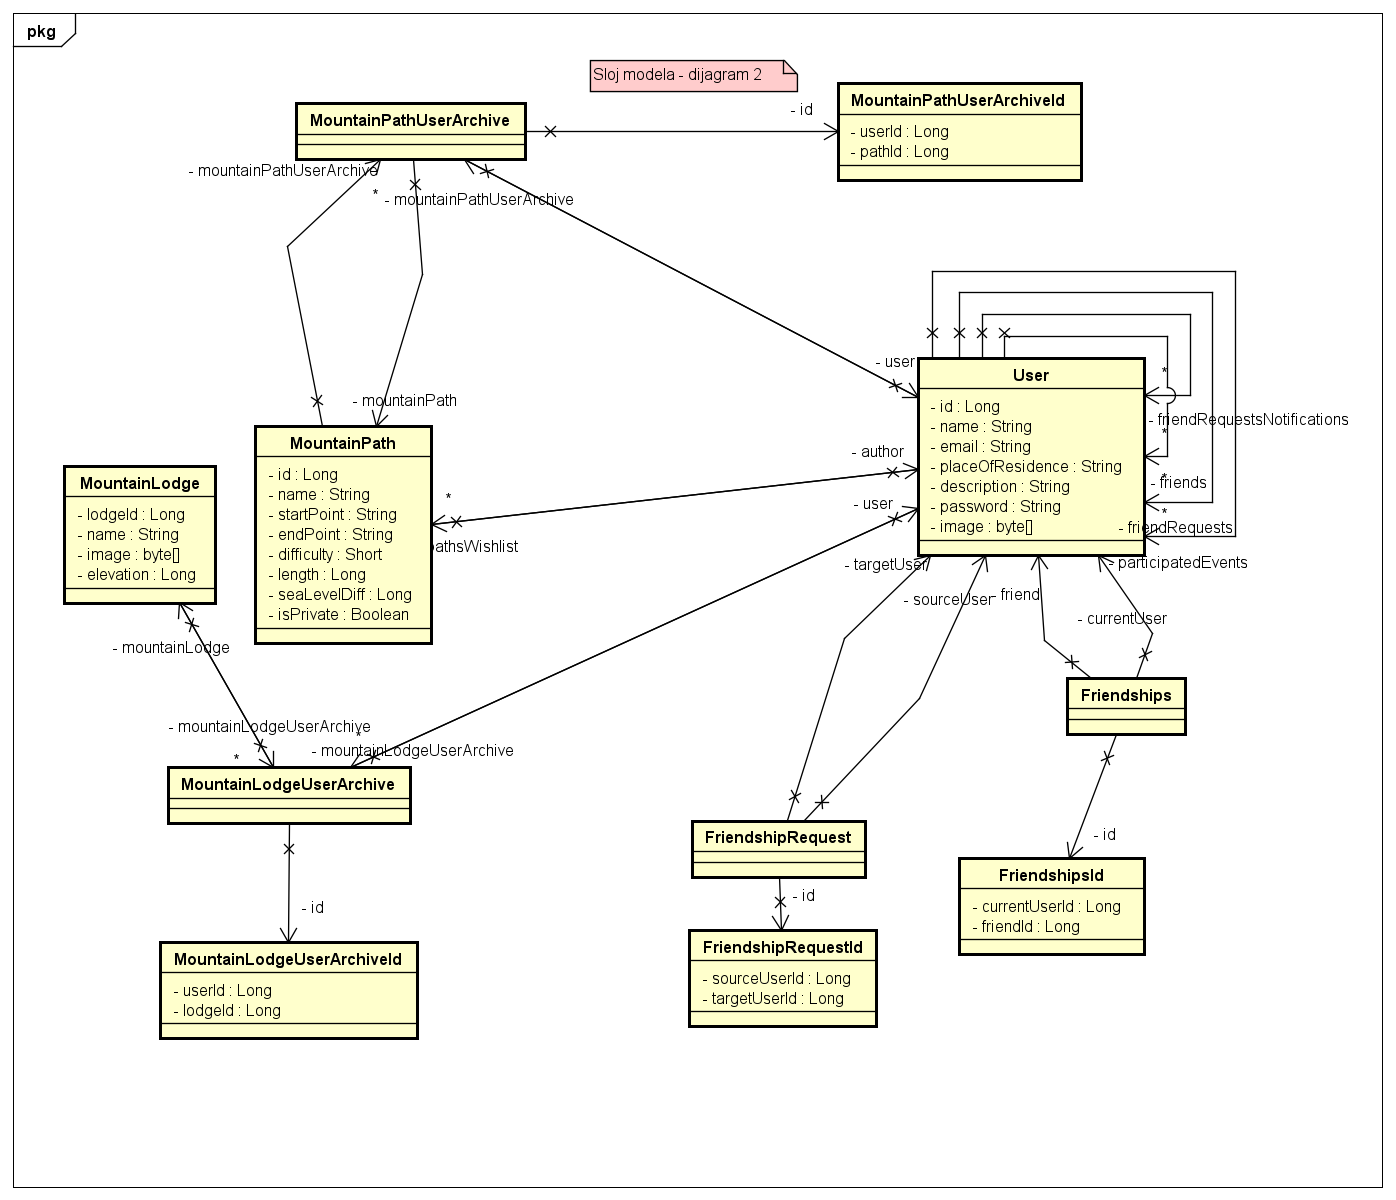
\includegraphics[scale=0.6, height=150mm, width=165mm]{dijagrami/model-dijagram2} %veličina slike u odnosu na originalnu datoteku i pozicija slike
			\centering
			\caption{Dijagram razreda - sloj modela drugi dijagram}
			\label{fig:dijagrami_razreda2}
		\end{figure}
			\newpage
			\subsubsection{Objekti za prijenos podataka i preslikavanja iz sloja modela}
			Na prvom od sljedeća dva dijagrama prikazani su objekti za prijenos podataka između klijenta i poslužitelja. Oni omogućuju da sloj nadglednika nikada ne komunicira sa stvarnim modelima. Iz imena DTO razreda možemo vidjeti za koji je razred taj objekt zadužen. Na drugom dijagramu prikazani su razredi koji služe za preslikavanje između sloja modela i objekata za prijenos podataka. Svi ti razredi implementiraju parametrizirano sučelje \textit{DefaultMapper}.
			\begin{figure}[H]
				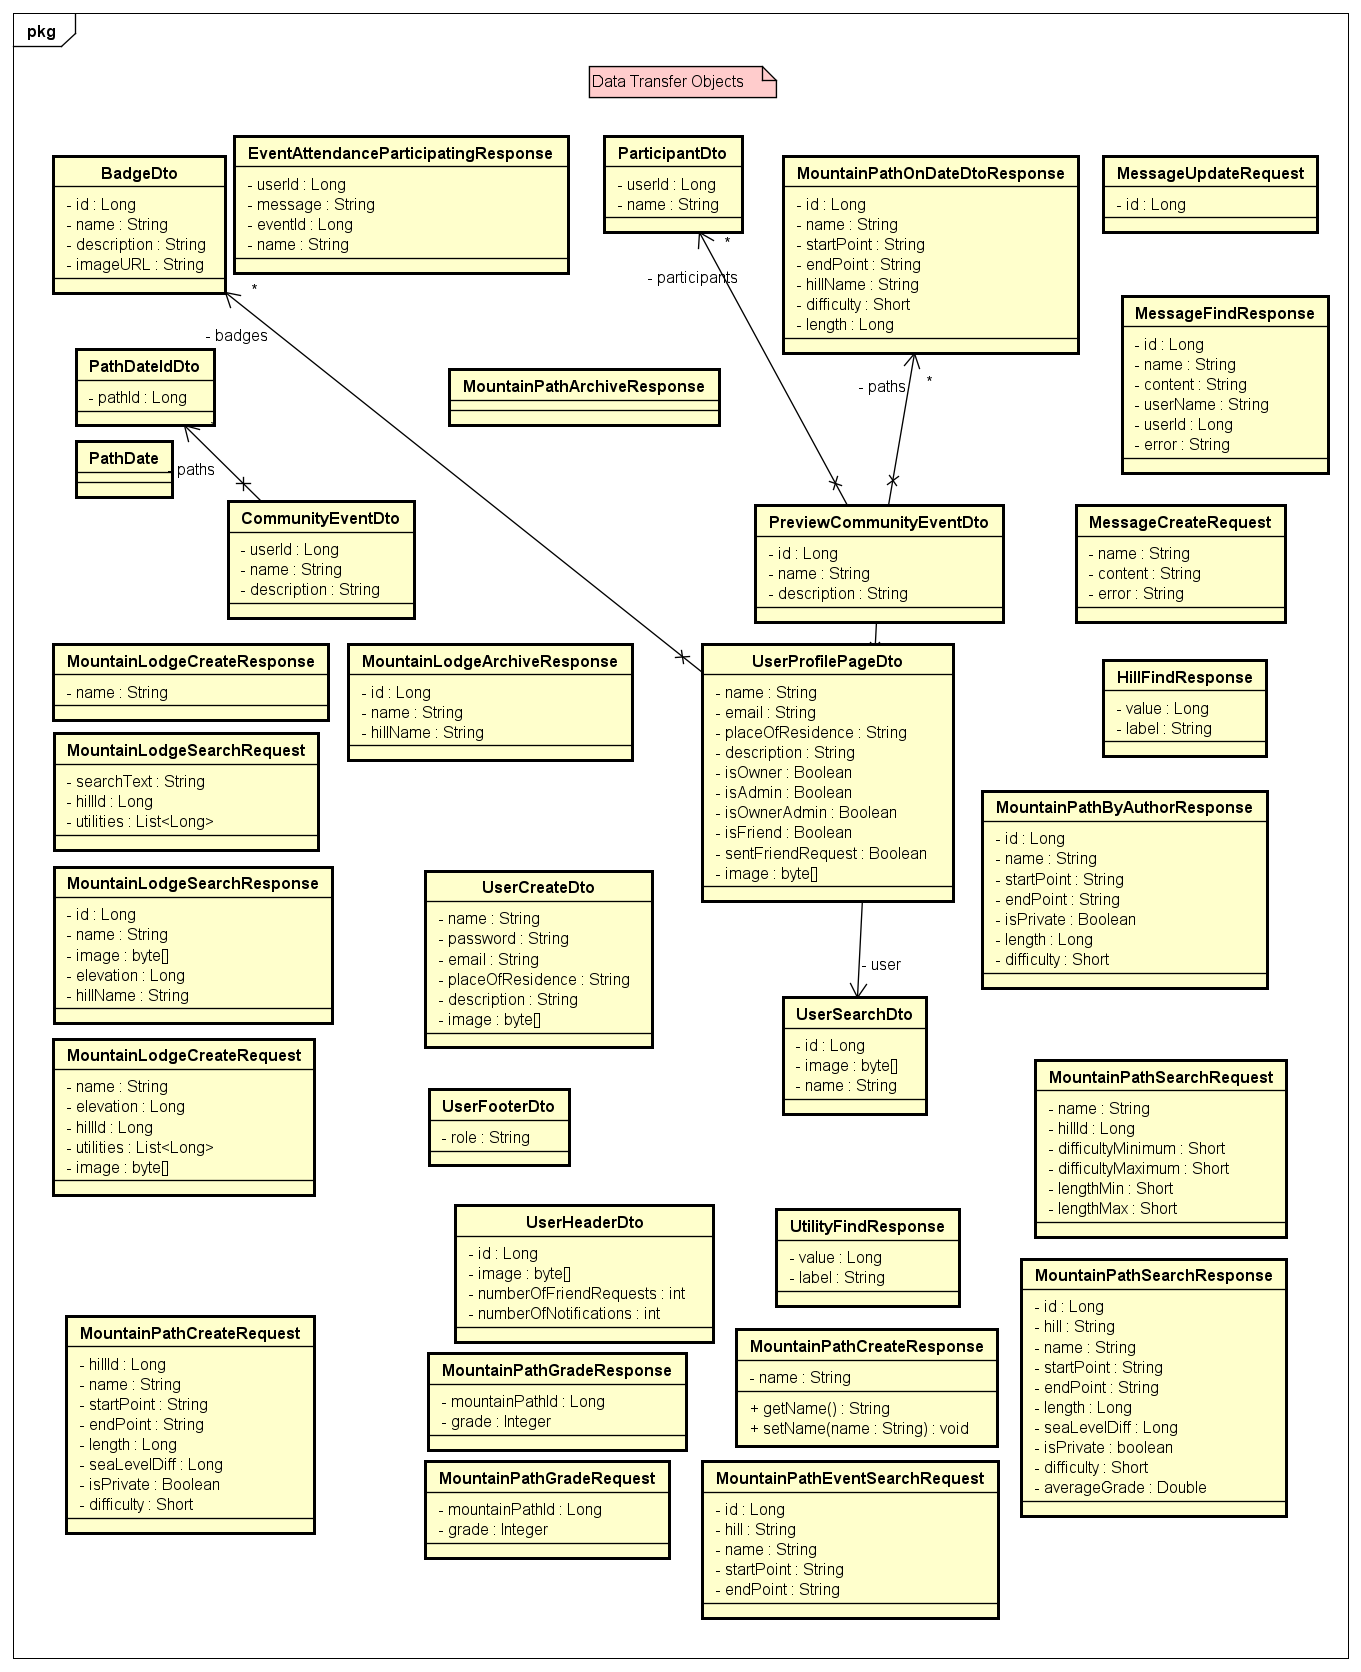
\includegraphics[scale=0.6, height=150mm, width=165mm]{dijagrami/dto-dijagram.png} %veličina slike u odnosu na originalnu datoteku i pozicija slike
				\centering
				\caption{Dijagram razreda - razredi za prijenos podataka}
				\label{fig:dijagrami_razreda3}
			\end{figure}
		\begin{figure}[H]
			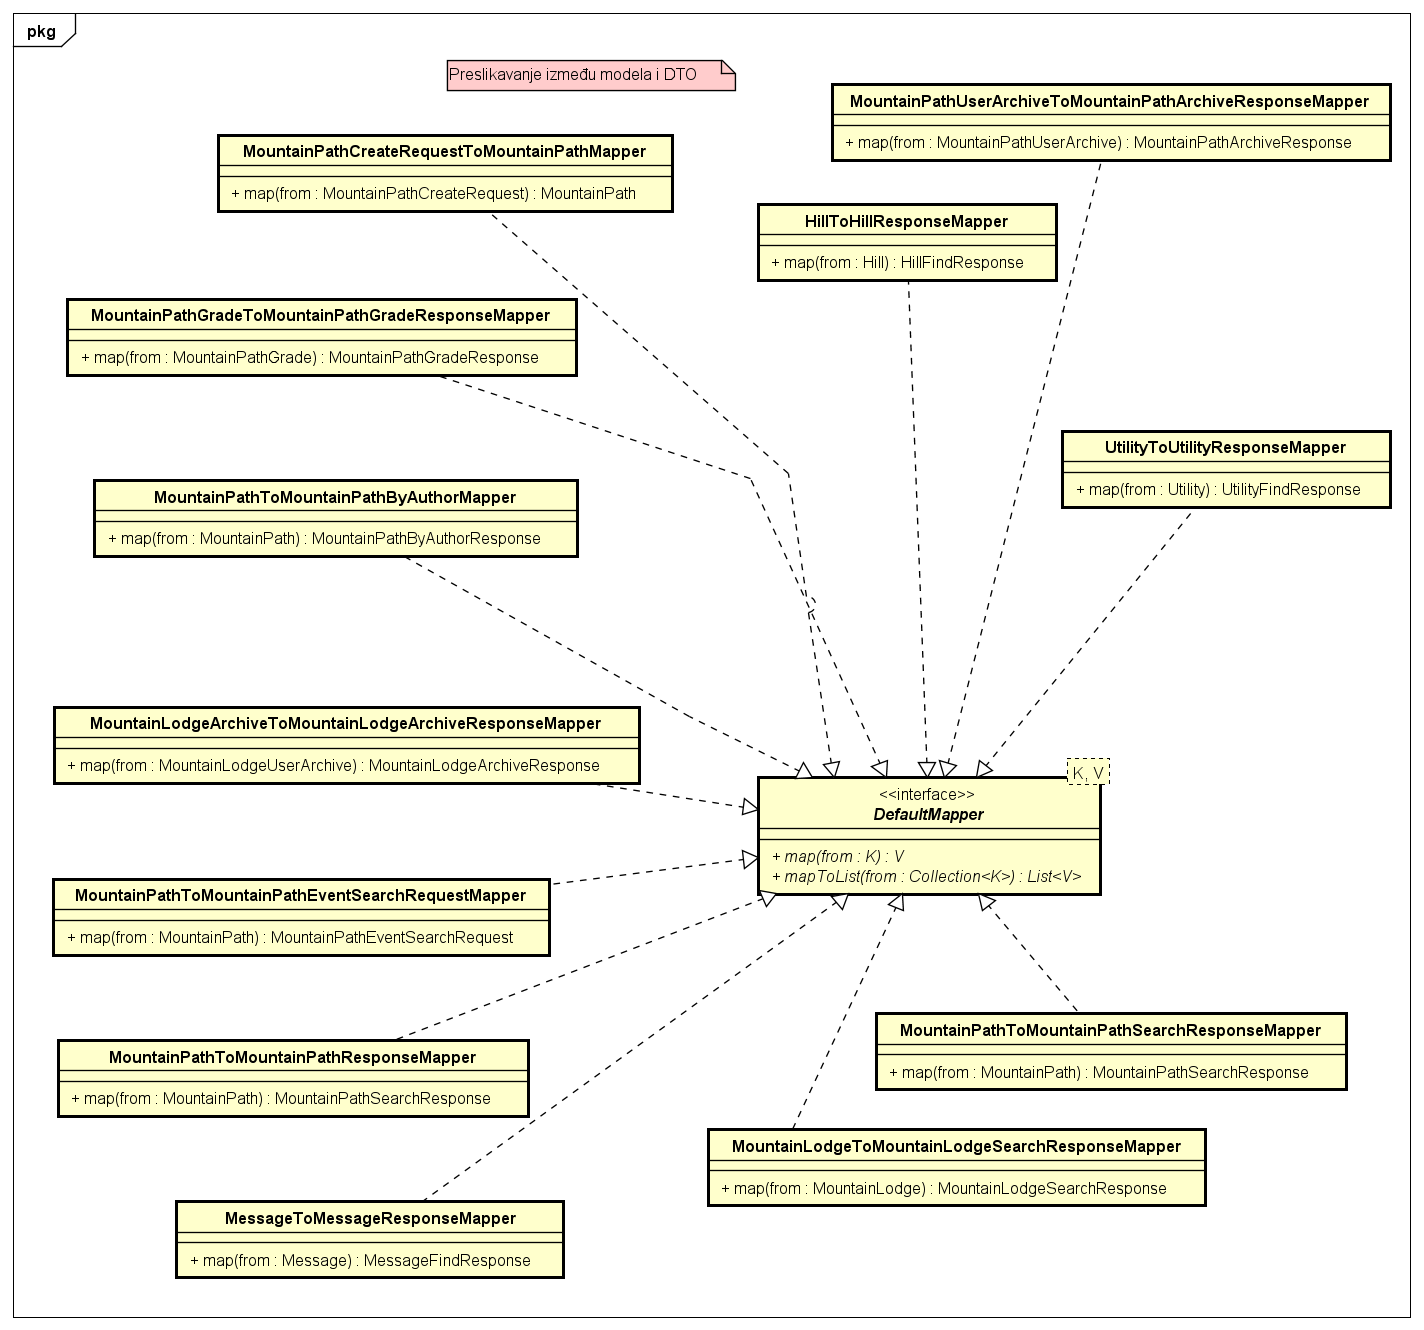
\includegraphics[scale=0.6, height=150mm, width=165mm]{dijagrami/model-mapper.png} %veličina slike u odnosu na originalnu datoteku i pozicija slike
			\centering
			\caption{Dijagram razreda - razredi za preslikavanje između sloja modela i DTO}
			\label{fig:dijagrami_razreda3}
		\end{figure}
			\newpage
			\subsubsection{Sloj nadglednik - servis - repozitorij}
			Ovaj sloj predstavlja sve operacije koje naš sustav obavlja. Razrađen je po oblikovnom obrascu "MVC". Zapravo se ovaj sloj sastoji od tri podsloja, a to su: 
			\begin{itemize}
				\item 
					Sloj repozitorija - metode pristupa bazi podataka, dohvat modela
				\item
					Sloj servisa - tu se obavlja sva naša poslovna logika, pozivaju se metode repozitorija dohvaćaju se podaci
				\item Sloj nadglednika - prima zahtjeve od korisnika i poziva metoda servisnog sloja	
			\end{itemize}
			Dijagram ovog sloja podijeljeni su na nekoliko manjih dijagrama.
			Razredi koji su trenutno implementirani u ovom sloju prikazani su na dijagramu slijedno, od najnižeg podsloja odnosno pristupa bazi podataka pa sve do podsloja nadglednika koji prima i delegira zahtjeve korisnika.
			Dijagrami se sastoje od nekoliko nadglednika: \textit{UserController}, \textit{MountainLodgeController}, \textit{MountainPathController}, \textit{HillController}, \textit{UtilityController}, \textit{MountainLodgeUserArchiveController}, \textit{MountainLodgePathArchiveController}, \textit{MessageController} te \textit{CommunityEventController}.
			
			Podsloj nadglednika povezan je sa servisnim slojem preko konkretnog primjerka razreda servisnog sloja kojeg čine razredi: \textit{UserService}, \textit{MountainLodgeQueryServiceImpl}, \textit{MountainPathQueryServiceImpl}, 
			\textit{HillQueryServiceImpl}, \textit{UtilityQueryServiceImpl}, \textit{UserDetailsServiceImpl}, \textit{UserBadgeServiceImpl}, \textit{MountainPathUserArchiveServiceImpl}, \textit{MountainLodgeUserArchiveServiceImpl}, \textit{MessageQueryServiceImpl} te \textit{CommunityEventService},
			 a oni predstavljaju implementacije odgovarajućih servisnih sučelja koji su također označeni na dijagramima.
			
			 Naposljetku, servisni sloj povezan je sa slojem repozitorija preko sučelja konkretnog repozitorija relevantnog za taj servis. U našem slučaju to su sučelja: \textit{BadgeRepository}, \textit{BadgeUserRepository}, \textit{CommunityEventMountainPathRepository}, \textit{CommunityEventRepository}, \textit{FriendshipRequestRepository}, \textit{FriendshipRepository}, \textit{HillRepository}, \textit{MessageRepository}, \textit{MountainLodgeRepository}, \textit{MountainLodgeUserArchiveRepository}, \textit{MountainPathGradeRepository}, \textit{MountainPathRepository}, \textit{MountainPathUserArchiveRepository}, \textit{RoleRepository}, \textit{UserRepository} te
			 \textit{UtilityRepository}. 
			 Svako sučelje repozitorija nasljeđuje sučelje \textit{JpaRepository} koje sadrži konkretnu implementaciju upita nad bazom podataka.
			 
			  Sučelje \textit{JpaSpecificationExecutor} omogućuje nam korištenje specifikacija \textit{MountainLodgeSearchSpecification} i \textit{MountainPathSearchSpecification} prilikom pretraživanja planinarskih domova i planinarskih staza iz baze podataka.
			\begin{figure}[H]
				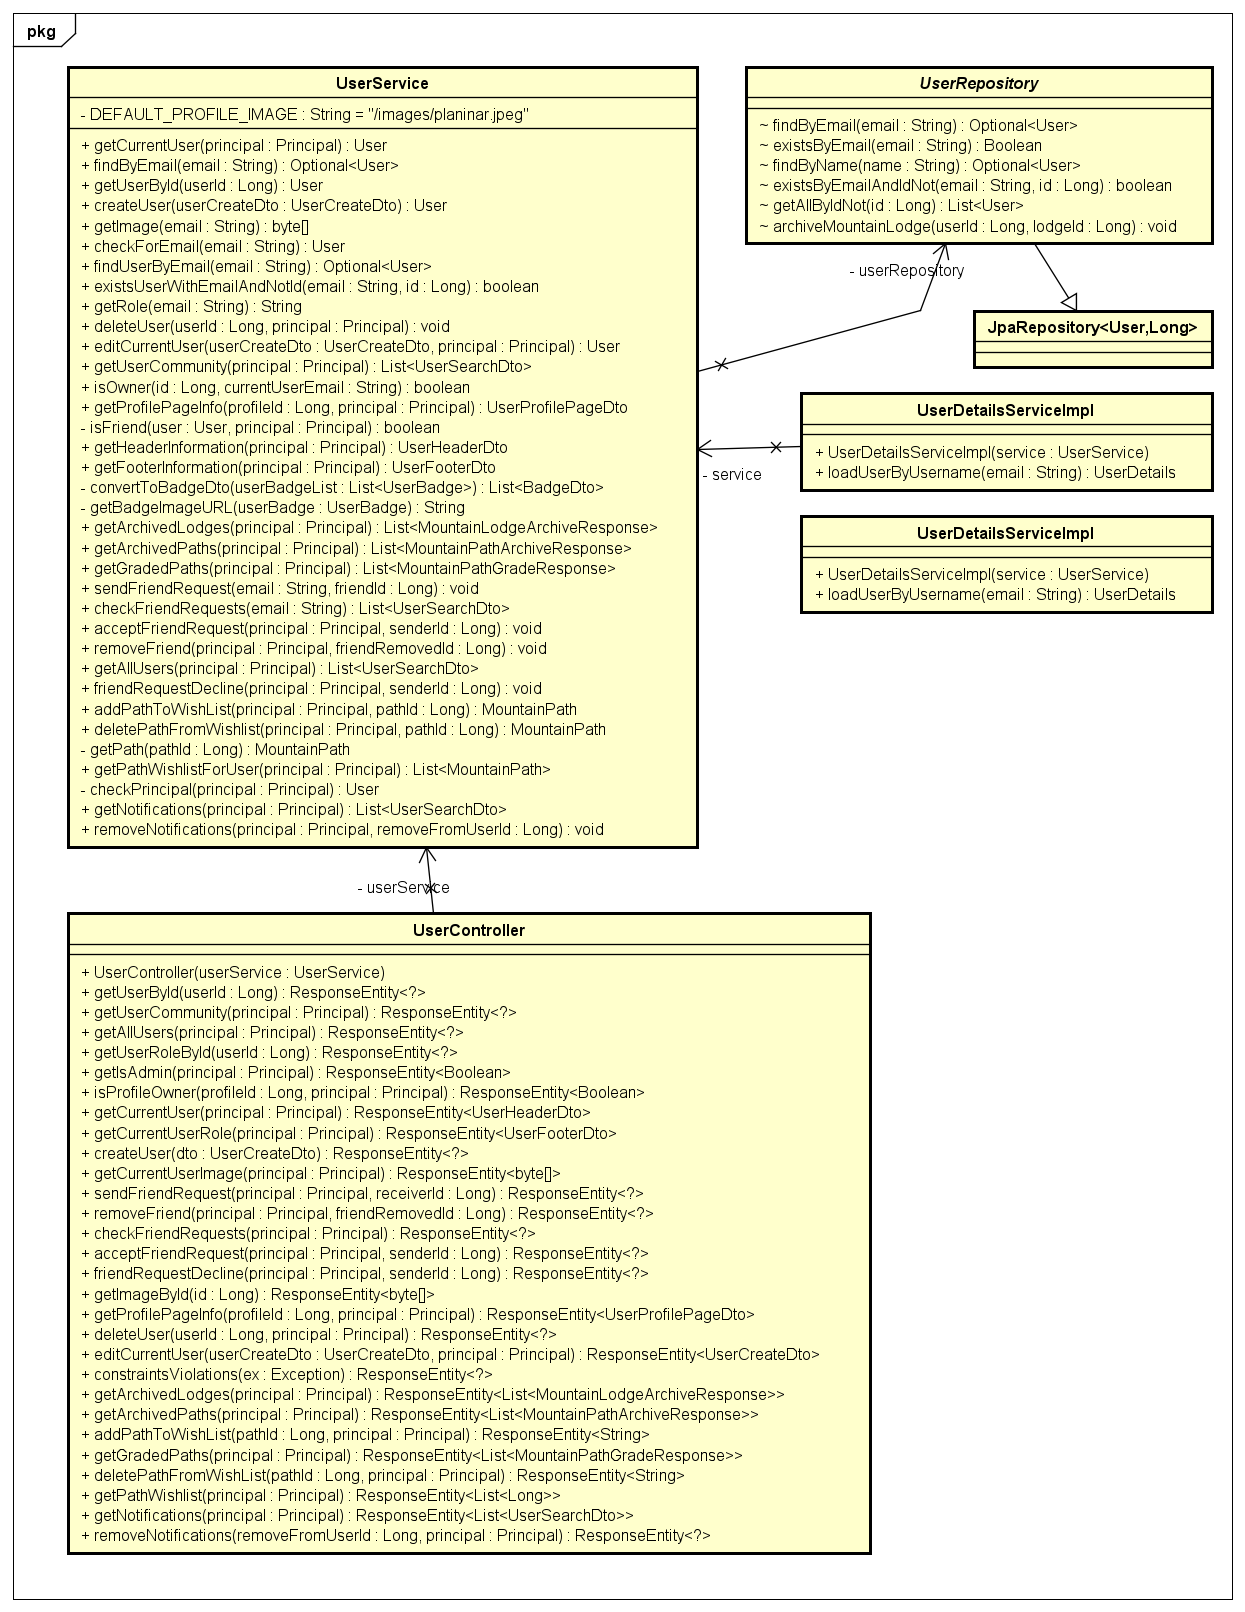
\includegraphics[scale=0.6, height=175mm, width=165mm]{dijagrami/csr-user-dijagram} %veličina slike u odnosu na originalnu datoteku i pozicija slike
				\centering
				\caption{Dijagram razreda korisnik - sloj nadglednik - servis - repozitorij}
				\label{fig:dijagrami_razreda_korisnik}
			\end{figure}
		\begin{figure}[H]
			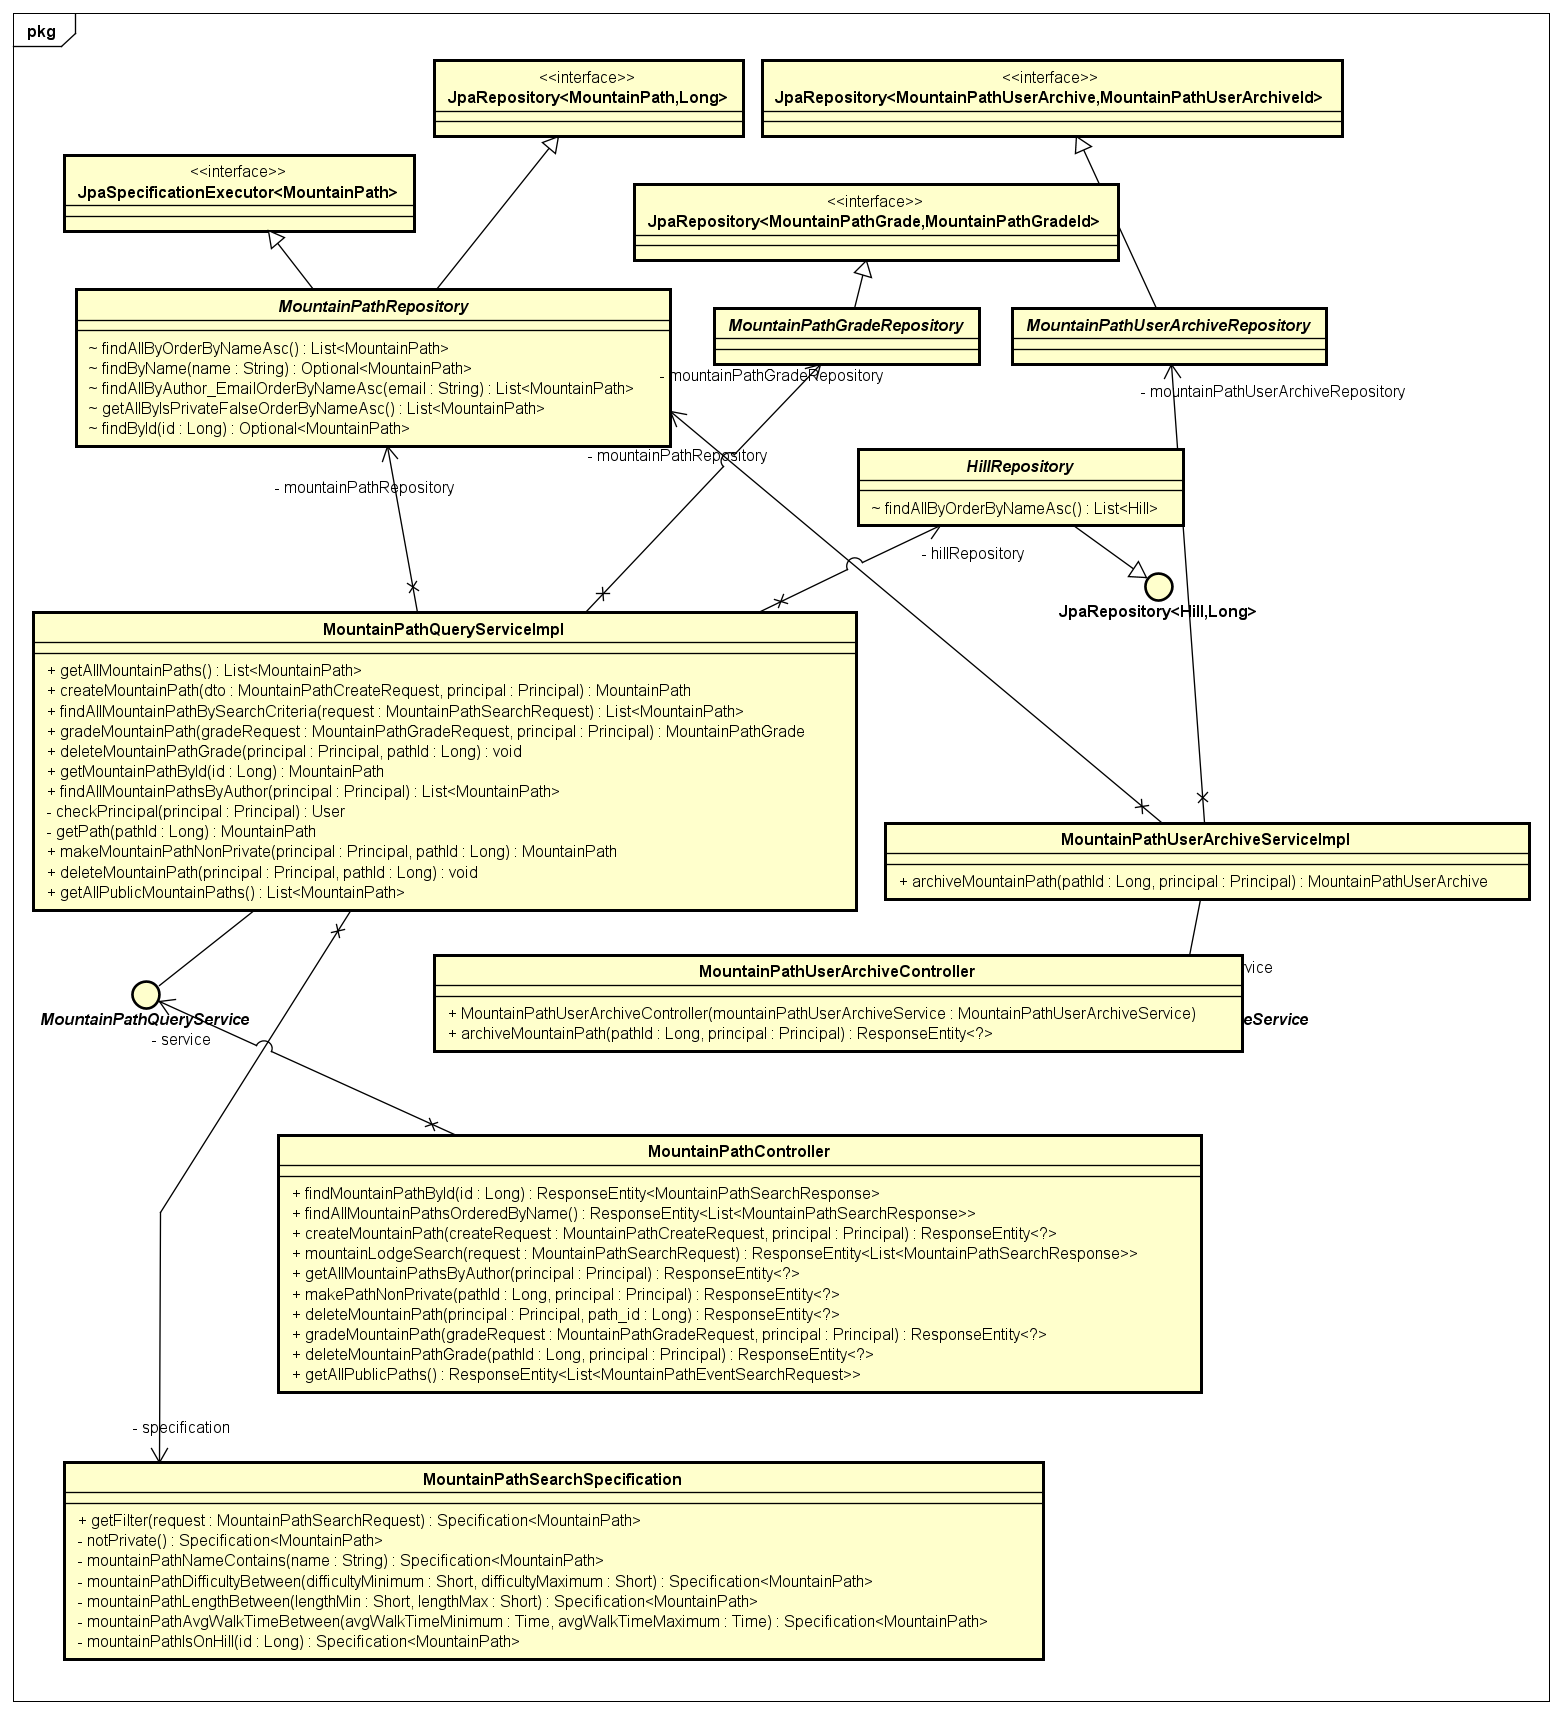
\includegraphics[scale=0.6, height=175mm, width=165mm]{dijagrami/csr-path-dijagram} %veličina slike u odnosu na originalnu datoteku i pozicija slike
			\centering
			\caption{Dijagram razreda planinarske staze - sloj nadglednik - servis - repozitorij}
			\label{fig:dijagrami_razreda_staze}
		\end{figure}
	\begin{figure}[H]
		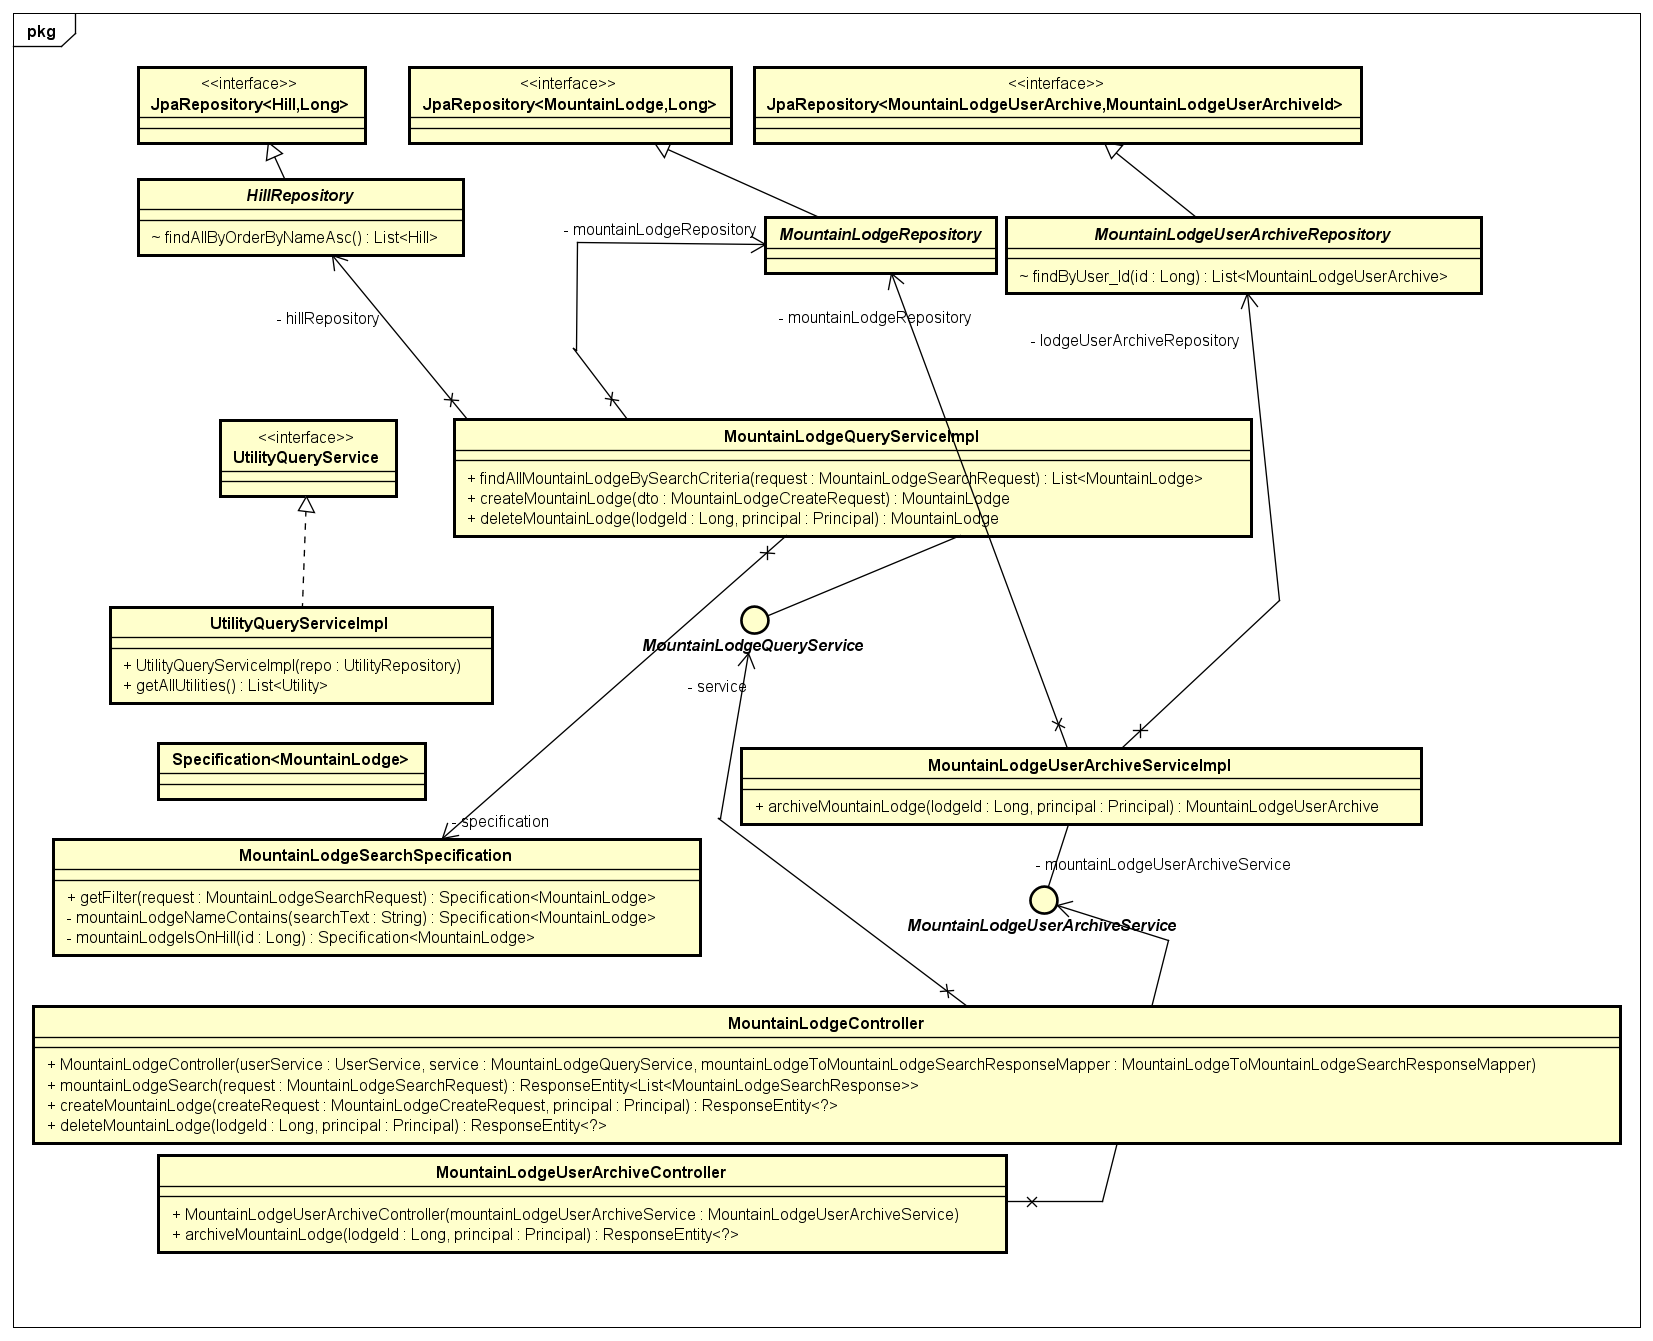
\includegraphics[scale=0.6, height=175mm, width=165mm]{dijagrami/csr-lodge-dijagram} %veličina slike u odnosu na originalnu datoteku i pozicija slike
		\centering
		\caption{Dijagram razreda planinarski dom - sloj nadglednik - servis - repozitorij}
		\label{fig:dijagrami_razreda_dom}
	\end{figure}	
		\begin{figure}[H]
			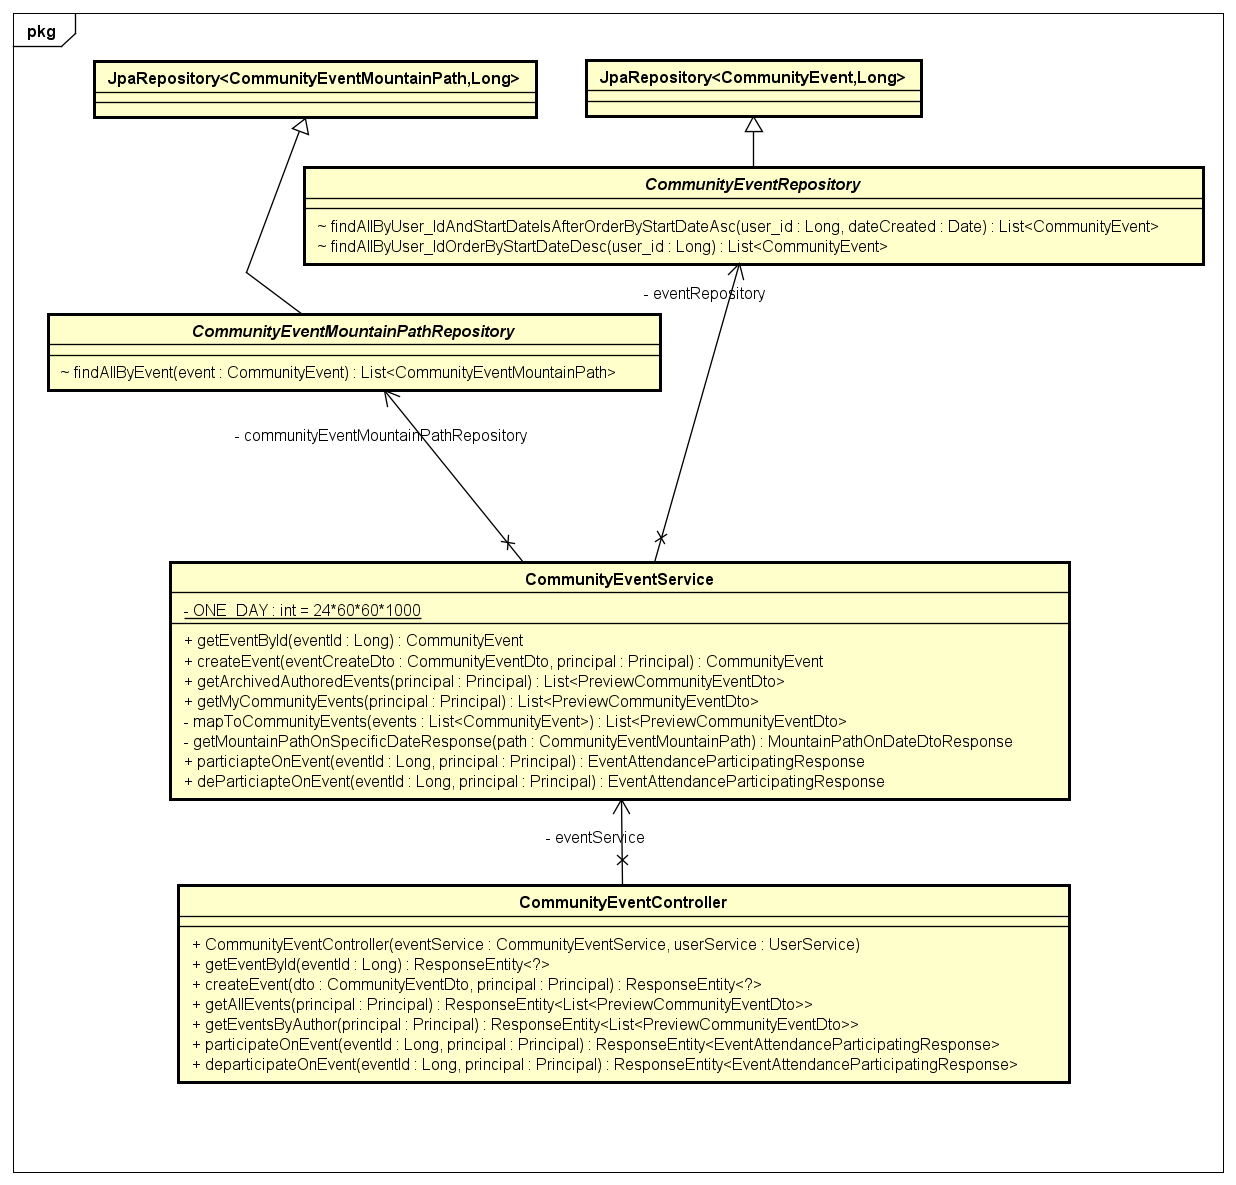
\includegraphics[scale=0.6, height=175mm, width=165mm]{dijagrami/csr-event-dijagram} %veličina slike u odnosu na originalnu datoteku i pozicija slike
			\centering
			\caption{Dijagram razreda planinarski događaji - sloj nadglednik - servis - repozitorij }
			\label{fig:dijagrami_razreda_dogadaj}
		\end{figure}
			\begin{figure}[H]
				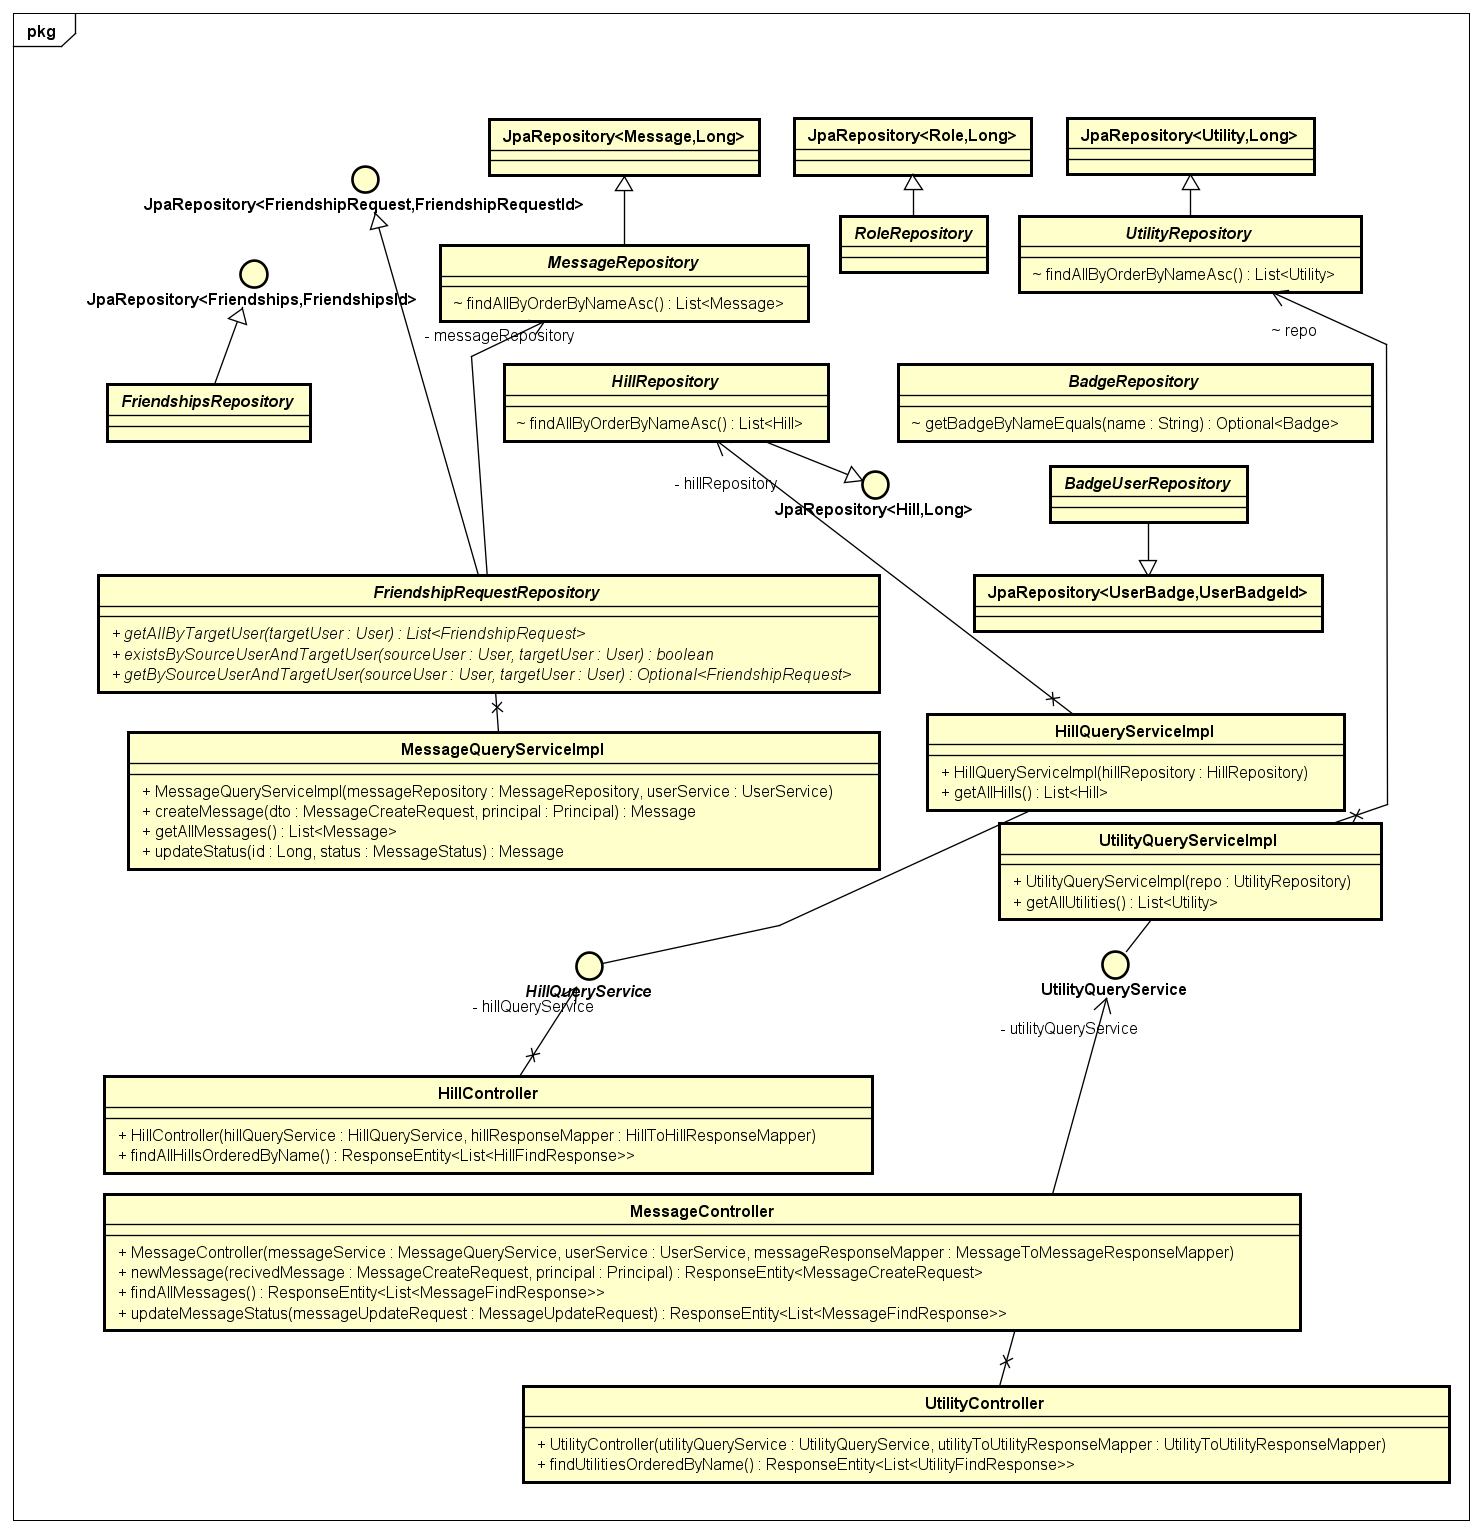
\includegraphics[scale=0.6, height=175mm, width=165mm]{dijagrami/csr-other-dijagram} %veličina slike u odnosu na originalnu datoteku i pozicija slike
				\centering
				\caption{Dijagram razreda, ostalo - sloj nadglednik - servis - repozitorij}
				\label{fig:dijagrami_razreda_ostalo}
			\end{figure}
			\newpage
			\subsubsection{Razredi vezani uz sigurnost i pomoćni razredi}
			Prilikom prijave korisnika, zahtjev za prijavu se šalje na back end, točnije do nadglednika. Zahtjev se provjerava u razredu \textit{JWTAuthenticationFilter} pomoću metode \textit{attemptAuthentication} koja stvara instancu razreda \textit{UserLogin} i šalje ga na provjeru.
			 
			 Provjera se vrši tako da se zove metoda \textit{loadUserByUsername} razreda \textit{UserDetailsServiceImpl}, a ona provjerava postoji li korisnik koji sadrži e-mail koji je poslan unutar zahtjeva. 
			 
			 Nakon utvrđivanja da ta osoba postoji \textit{Spring security modul} provjerava lozinku i druge podatke vezane uz prijavu. Nakon uspješne prijave pomoću metode \textit{successfulAuthentication} se generira jedinstveni token (identifikator) i šalje korisniku. Svojstva tokena poput trajanja se određuju u razredu \textit{SecurityConstants}. 
			
			Prijavljeni korisnik za vrijeme rada unutar Web aplikacije svaki zahtjev obavlja pomoću jedinstvenog tokena koji mu je dodijeljen, a koji se provjerava unutar razreda \textit{JWTAuthorizationFilter}. 
			
			Metoda \textit{getPasswordEncoder} razreda \textit{Configuration} služi da bi definirali enkoder za zaštitu lozinki. 
			
			Razred \textit{UniqueEmailValidator} prilikom registracije provjerava postoji li u bazi podataka korisnik kojem je e-mail isti e-mailu zahtjeva. Budući da ne možemo imati dva korisnika s istom adresom elektroničke pošte, u tom slučaju događa se iznimka \textit{UserWithEmailExistsException}.
			
			Na drugom dijagramu prikazane su iznimke koje je moguće izazvati na poslužiteljskoj strani, kao i razred koji obrađuje iznimke.  
		
			\begin{figure}[H]
				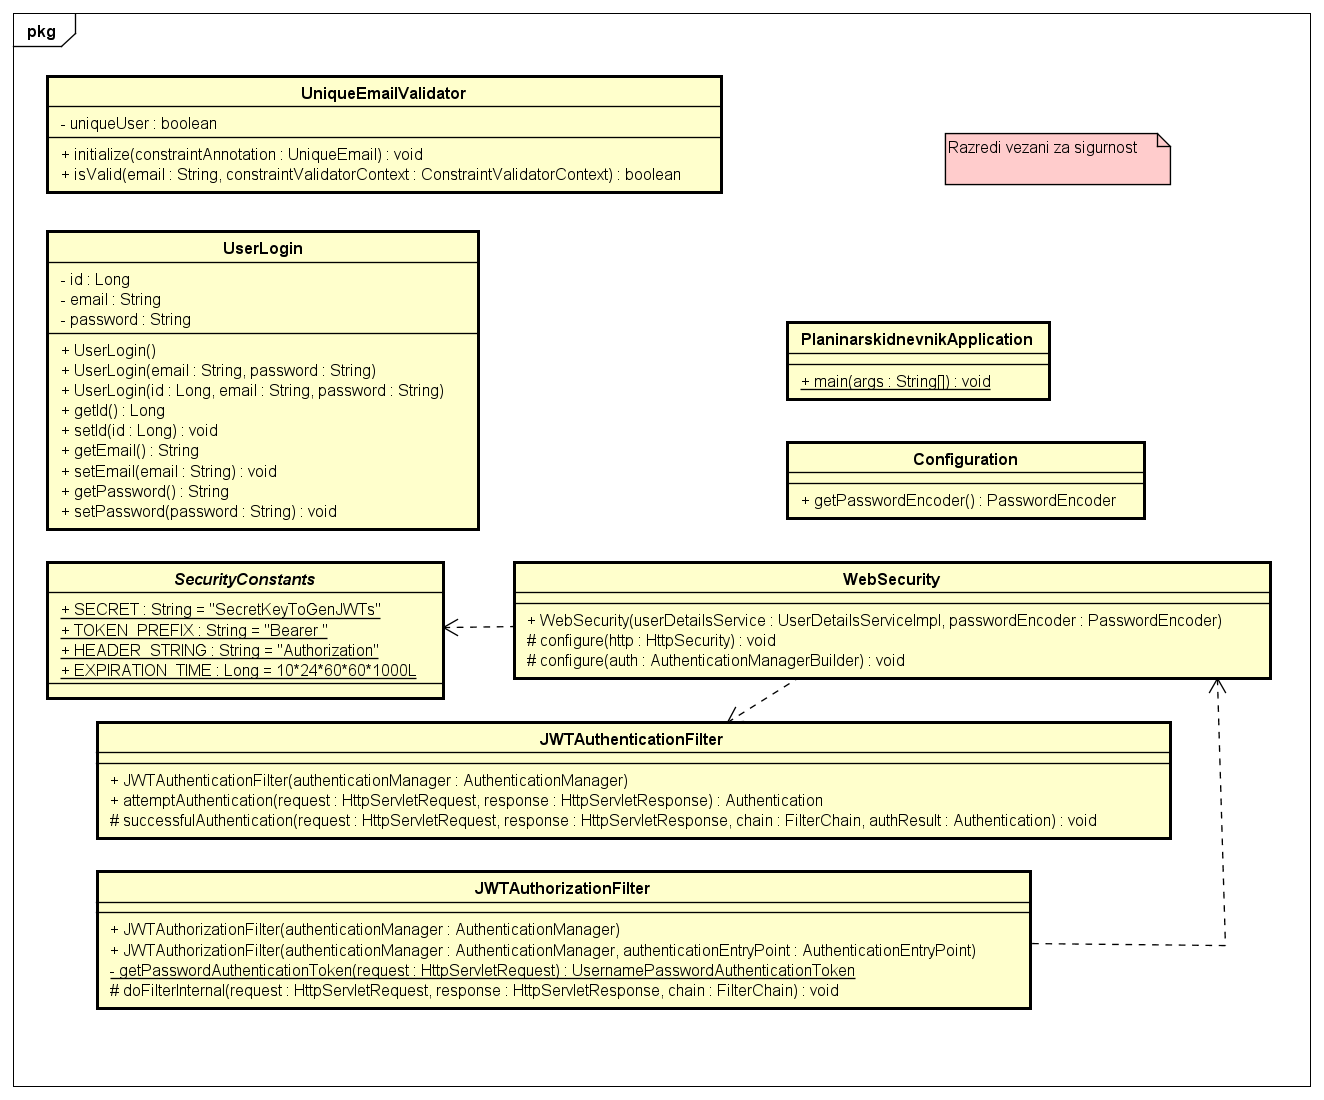
\includegraphics[scale=0.6, height=175mm, width=165mm]{dijagrami/helpers-class.png} %veličina slike u odnosu na originalnu datoteku i pozicija slike
				\centering
				\caption{Dijagram razreda - sigurnost}
				\label{fig:dijagrami_razreda5}
			\end{figure}
		
		\begin{figure}[H]
			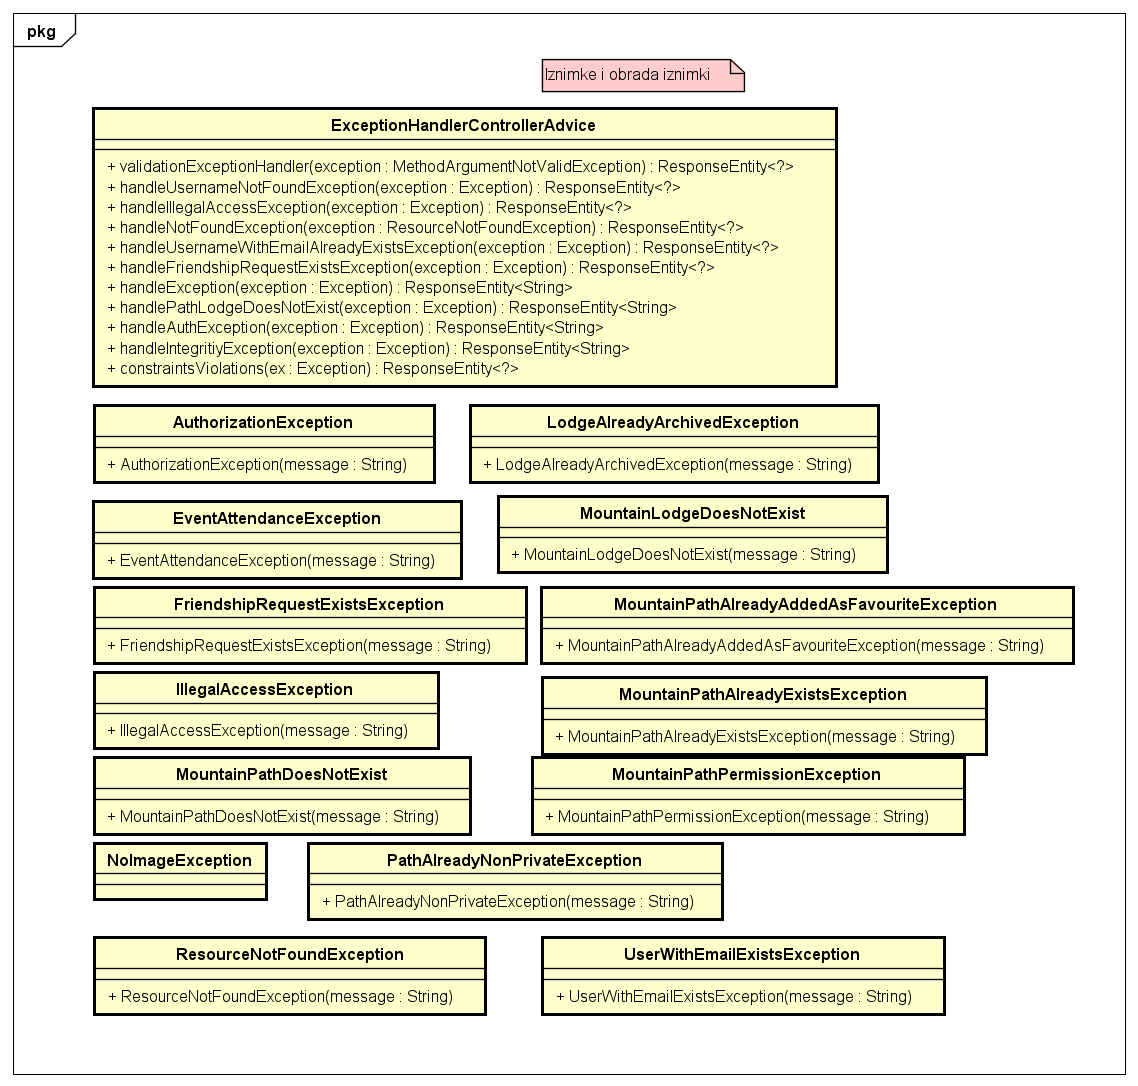
\includegraphics[scale=0.6, height=175mm, width=165mm]{dijagrami/iznimke-dijagram.png} %veličina slike u odnosu na originalnu datoteku i pozicija slike
			\centering
			\caption{Dijagram razreda - iznimke i upravljanje iznimkama}
			\label{fig:dijagrami_razreda5}
		\end{figure}
			
			\eject
			
			
			
			
			\eject
		
		\section{Dijagram stanja}
			
		
			Dijagrami stanja prikazuju stanja objekata i njihov prelazak iz jednog stanja u drugo. Takav pogled nam dozvoljava veću preglednost sustava. Zbog čitljivosti smo mi naše dijagrame stanja podijelili u više odvojenih dijagrama. 
			
			Na slici 4.9 prikazan je proces autentikacije. Korisnik dolazi u aplikaciju u neprijavljenom stanju. Iz toga stanja može vršiti određene akcije, poput pregledavanja domova i staza. Da mu se omogući pregled profila, kreiranje staza i ako je admin, kreiranje domova, mora se ulogirati/registrirati. Taj proces je prikazan na dijagramu. Klikom na "log in" korisnik prelazi u stanje ulogiranja. Ako unese pogrešne informacije, stanje se resetira. Ako klikne na "nemate račun", otići će na stranicu registracije. Ako unese pogrešne podatke, stanje mu se resetira. Na registraciju može otići i direktno iz headera. Kada se uspješno registrira, vraća ga na log in. Kada se ulogira, onda ima globalno stanje "prijavljen" što mu omogućava pristup većem broju sadržaja same stranice.
			
			\begin{figure}[H]
				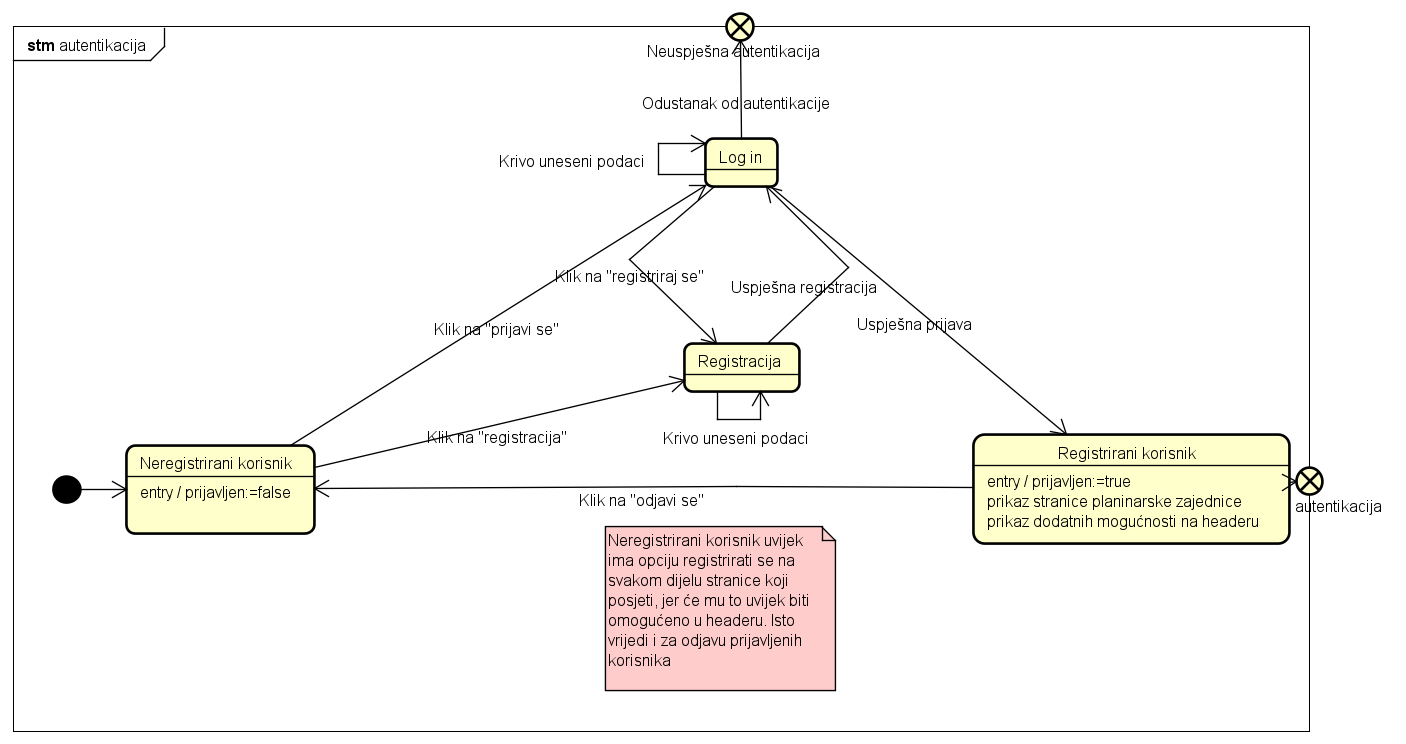
\includegraphics[width=160mm,height=100mm]{dijagrami/sd-autentikacija/autentikacija.png} %veličina slike u odnosu na originalnu datoteku i pozicija slike
				\centering
				\caption{Dijagram stanja - autentikacija}
				\label{fig:dijagrami_stanja1}
			\end{figure}
			\newpage
			Na slici 4.10 prikazana su stanja vezana za domove. Početno stanje provjerava je li korisnik admin, i ako je, prikazuje mu gumb za kreiranje domova. Ako korisnik nije admin, ne prikazuje mu se taj gumb i ne može kreirati domove, samo pregledavati. Prijavljenom korisniku se još prikazuju gumbi za arhiviranje staze i prijavljivanje pogreške na stazi
			
			\begin{figure}[H]
				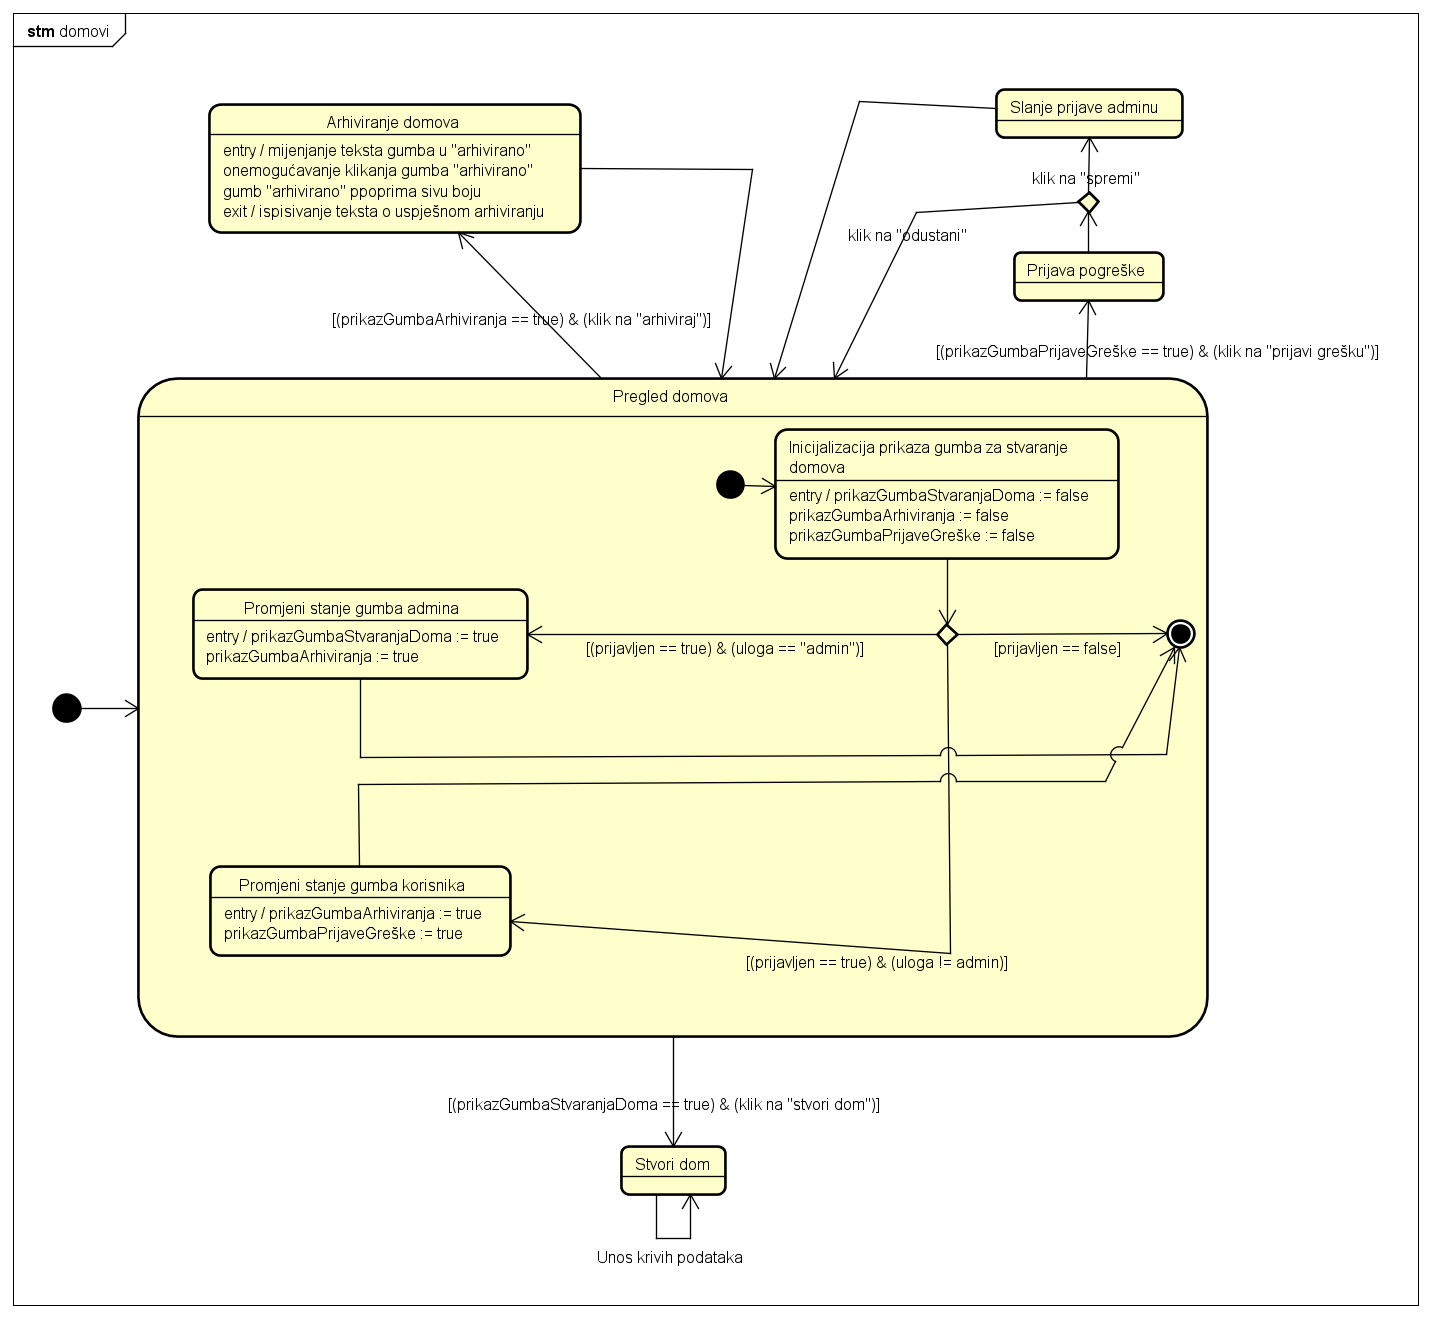
\includegraphics[width=160mm,height=150mm]{dijagrami/sd-autentikacija/domovi.png} %veličina slike u odnosu na originalnu datoteku i pozicija slike
				\centering
				\caption{Dijagram stanja - domovi}
				\label{fig:dijagrami_stanja2}
			\end{figure}
		
		    Na slici 4.11 prikazana su stanja vezana za planinarske staze. Početno stanje provjerava je li korisnik prijavljen, i ako je, prikazuje mu gumb za kreiranje staza. Ako korisnik nije prijavljen, ne prikazuje mu se taj gumb i ne može kreirati staze, samo pregledavati. Dodatno se prijavljenom korisniku prikazuju gumbi za dodavanje u favorite, ocjenjivanje staze, arhiviranje staze i prijavljivanje pogreške na stazi
		    
		    \begin{figure}[H]
		    	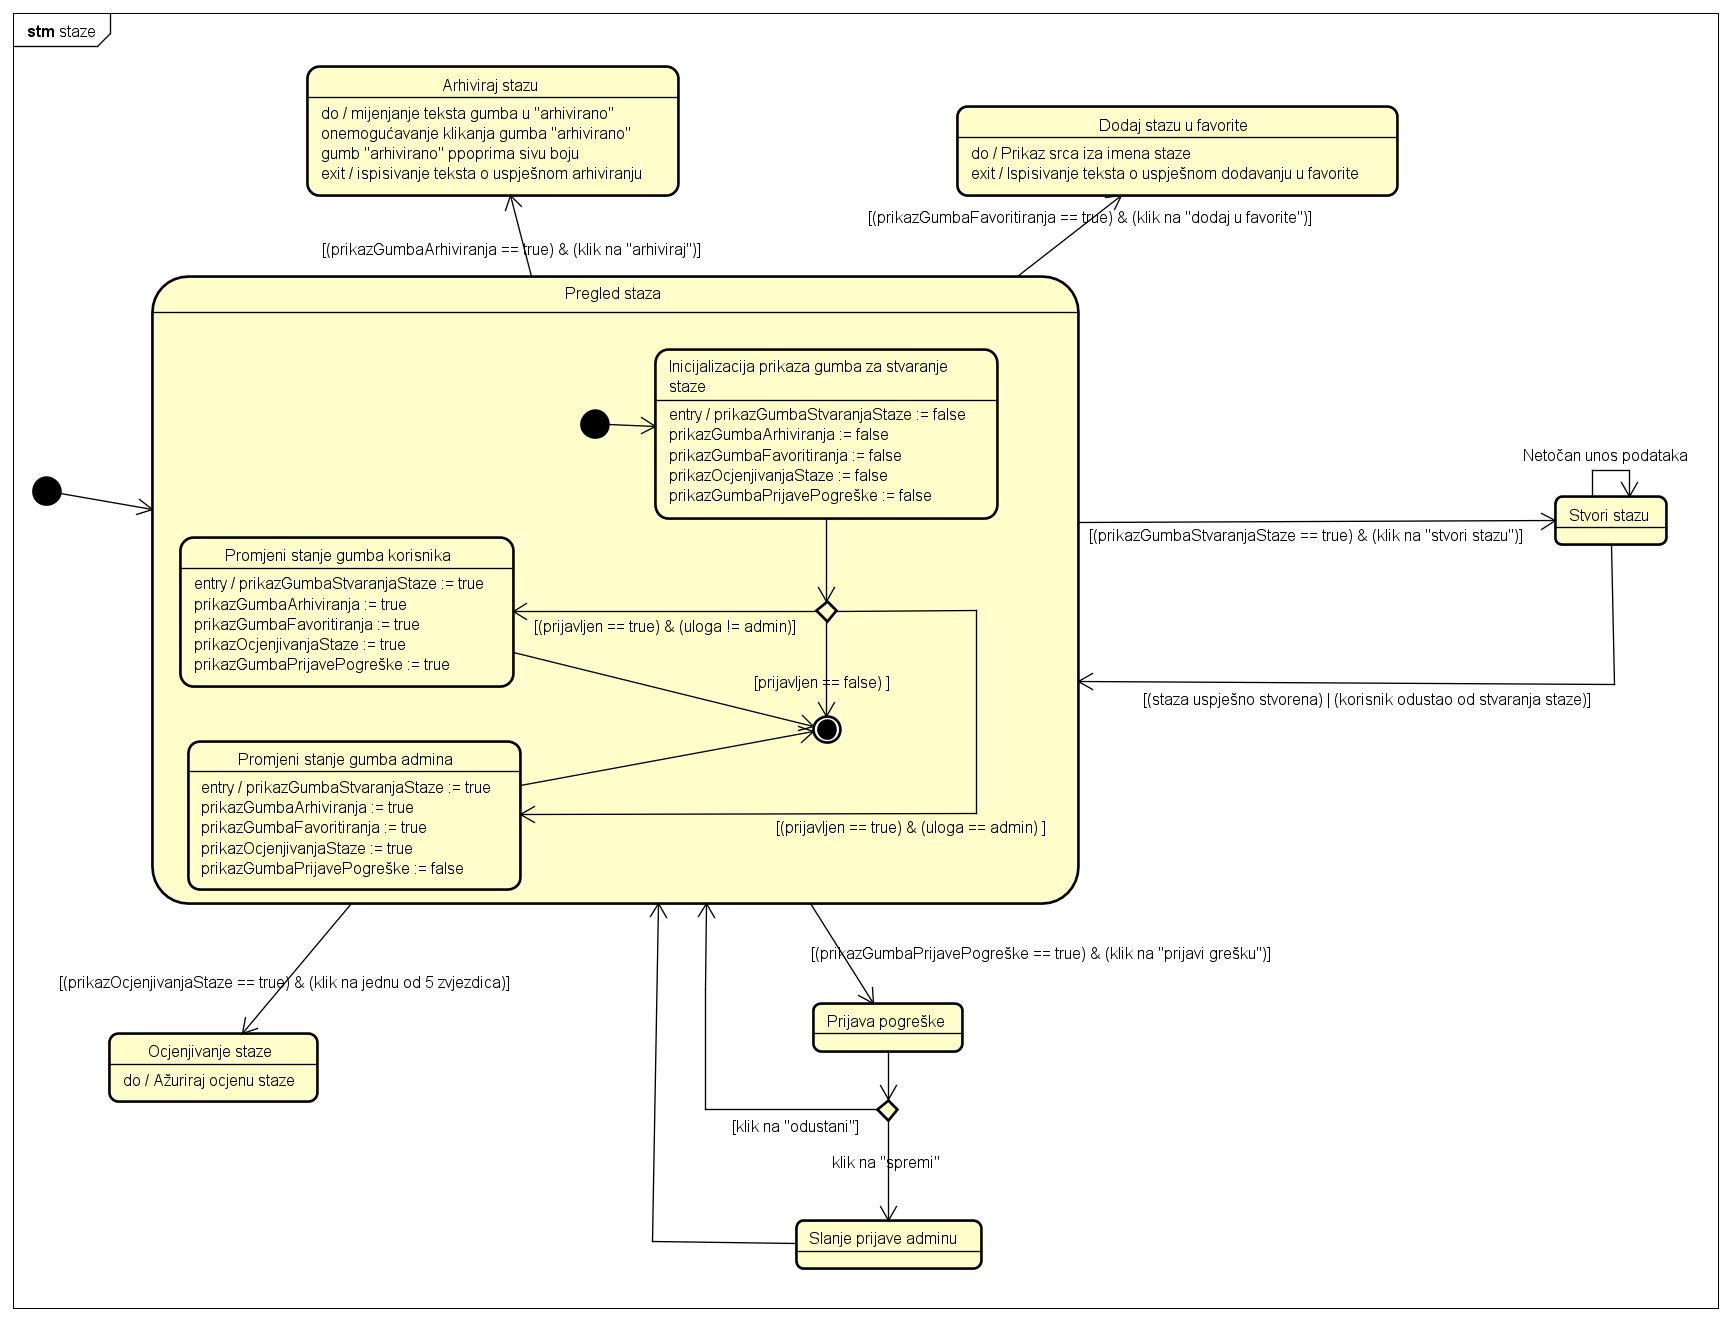
\includegraphics[width=160mm, height=160mm]{dijagrami/sd-autentikacija/staze.png} %veličina slike u odnosu na originalnu datoteku i pozicija slike
		    	\centering
		    	\caption{Dijagram stanja - staze}
		    	\label{fig:dijagrami_stanja3}
		    \end{figure}
			
			\newpage
			Na slici 4.12 prikazana su stanja vezana za korisnički profil. Ako je prijavljen, korisnik može otići na svoj profil gdje su mu omogućene radnje poput pregleda profila, uređivanje vlastitog profila, pretraživanja planinarske zajednice, brisanje profila i potvrda brisanja profila.
			
			\begin{figure}[H]
				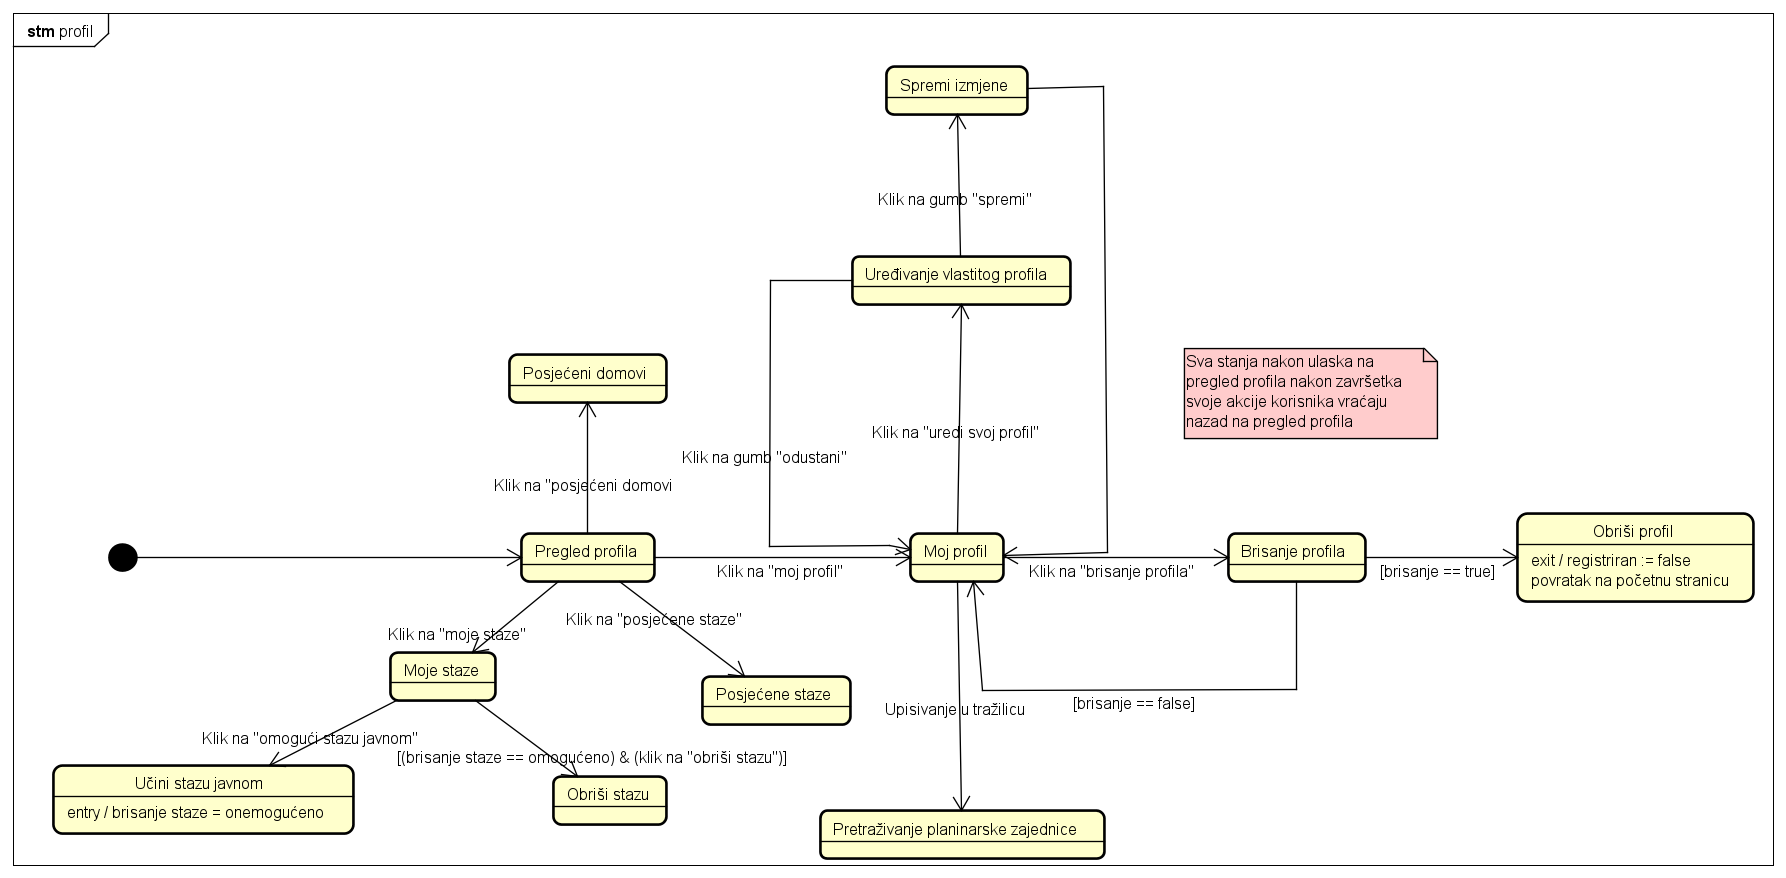
\includegraphics[width=160mm, height=165mm]{dijagrami/sd-autentikacija/profil.png} %veličina slike u odnosu na originalnu datoteku i pozicija slike
				\centering
				\caption{Dijagram stanja - profil}
				\label{fig:dijagrami_stanja4}
			\end{figure}
			
			\eject 
			

		
		\section{Dijagram aktivnosti}
			
			 Dijagram aktivnosti se koristi za modeliranje poslovnih procesa, upravljačkog i podatkovnog toka. Pogodni su za opisivanje sinkronizacije i konkurentnosti. Ne primjenjuju se za modeliranje događajima poticanog ponašanja. Na dijagramu 4.13 prikazan je dijagram aktivnosti pretrage i arhiviranja staze. U našoj aplikaciji, jedna od funkcionalnosti koju dozvoljavamo korisniku je pretraga planinarskih staza po nekim parametrima, prikaz detalja o toj stazi i mogućnost arhiviranja te staze kako bi korisnik mogao čuvati informaciju o stazama koje je prešao. Ako je arhivirao određeni broj staza, dobiva bedž na svome profilu koji to označava.
			 
			 \begin{figure}[H]
			 	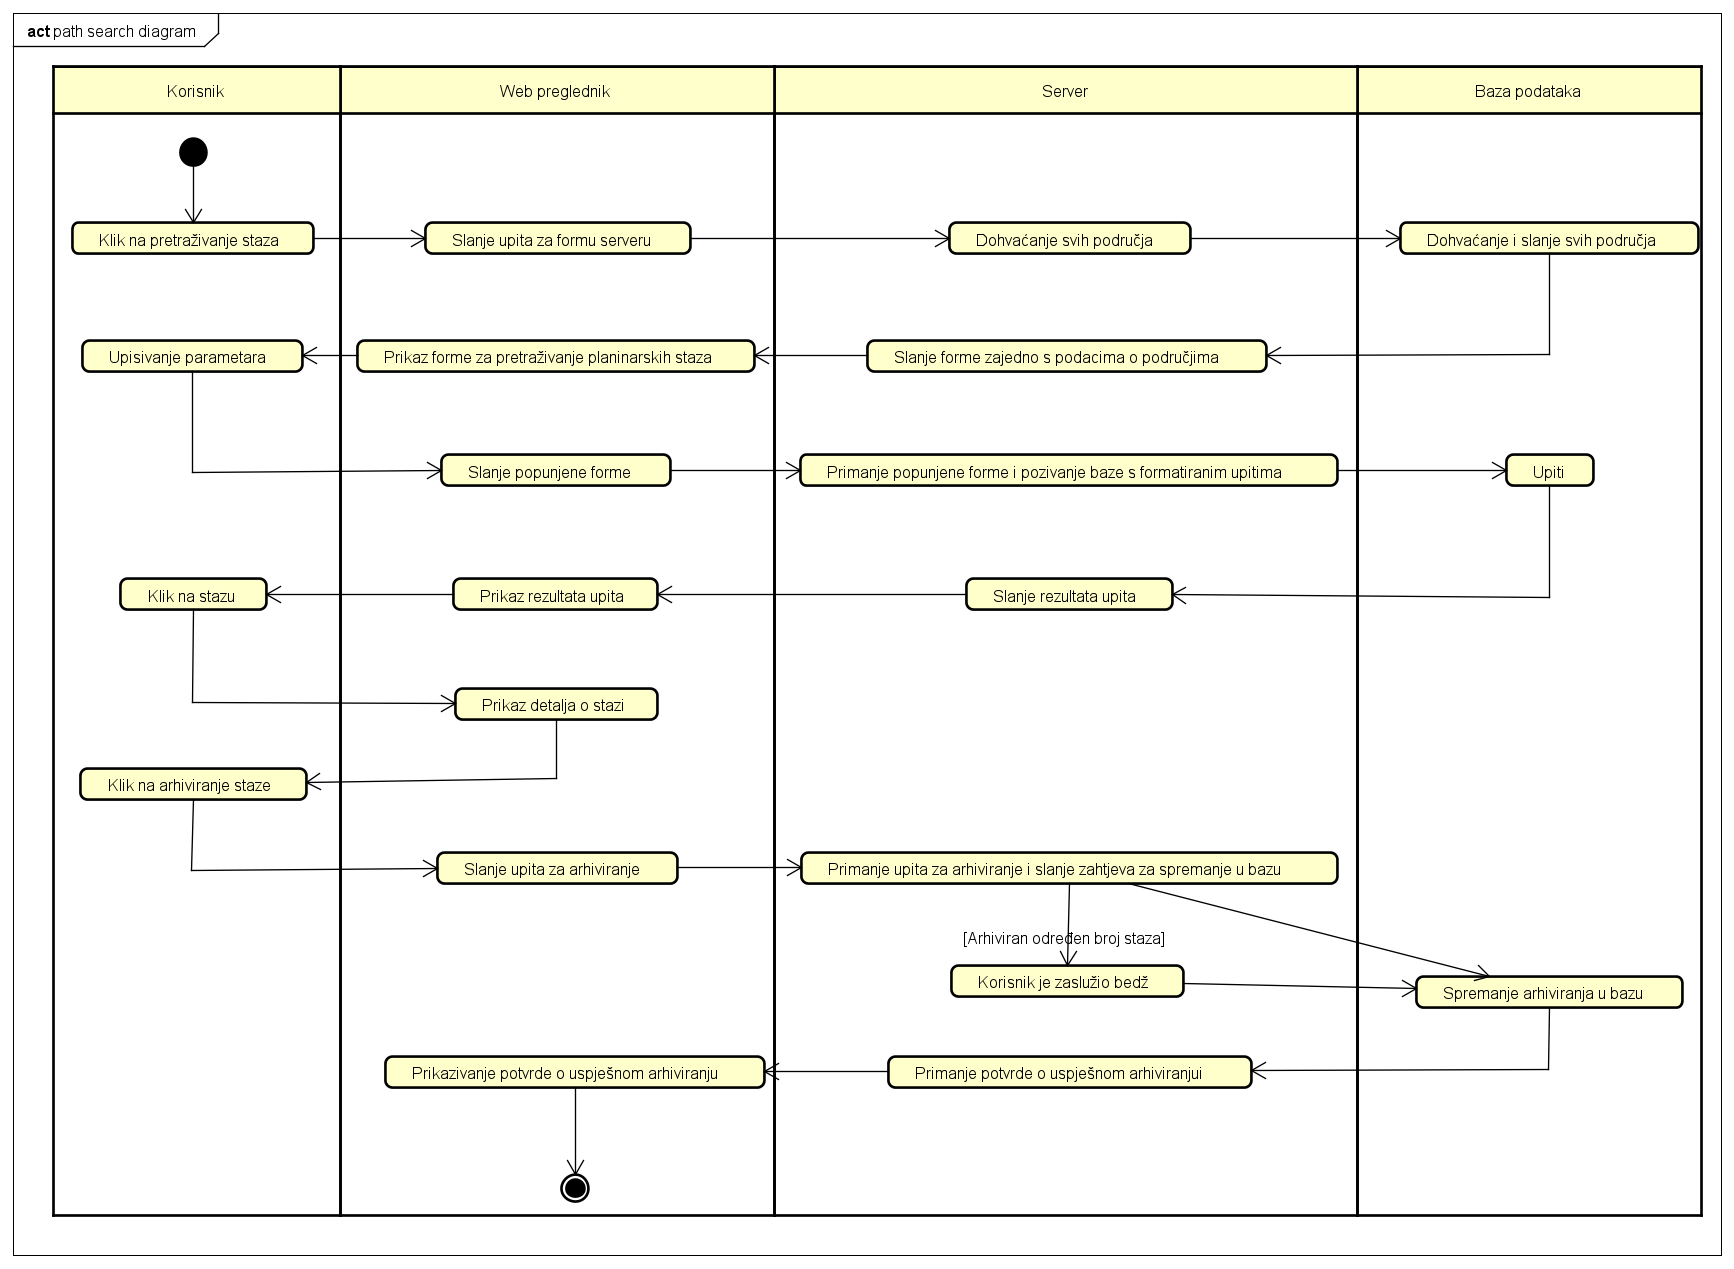
\includegraphics[scale=0.6, height=150mm, width=165mm]{dijagrami/activity/path search diagram.png} %veličina slike u odnosu na originalnu datoteku i pozicija slike
			 	\centering
			 	\caption{Dijagram aktivnosti - pretraga i arhiviranje staze}
			 	\label{fig:dijagrami_aktivnosti1}
			 \end{figure}
		 
		 	Još jedna od funkcionalnosti je dodavanje prijatelja. Korisnik može Poslati zahtjev za prijateljstvo drugom korisniku. Taj drugi korisnik nakon toga može prihvatiti ili odbiti zahtjev za prijateljstvo
		 	\begin{figure}[H]
		 	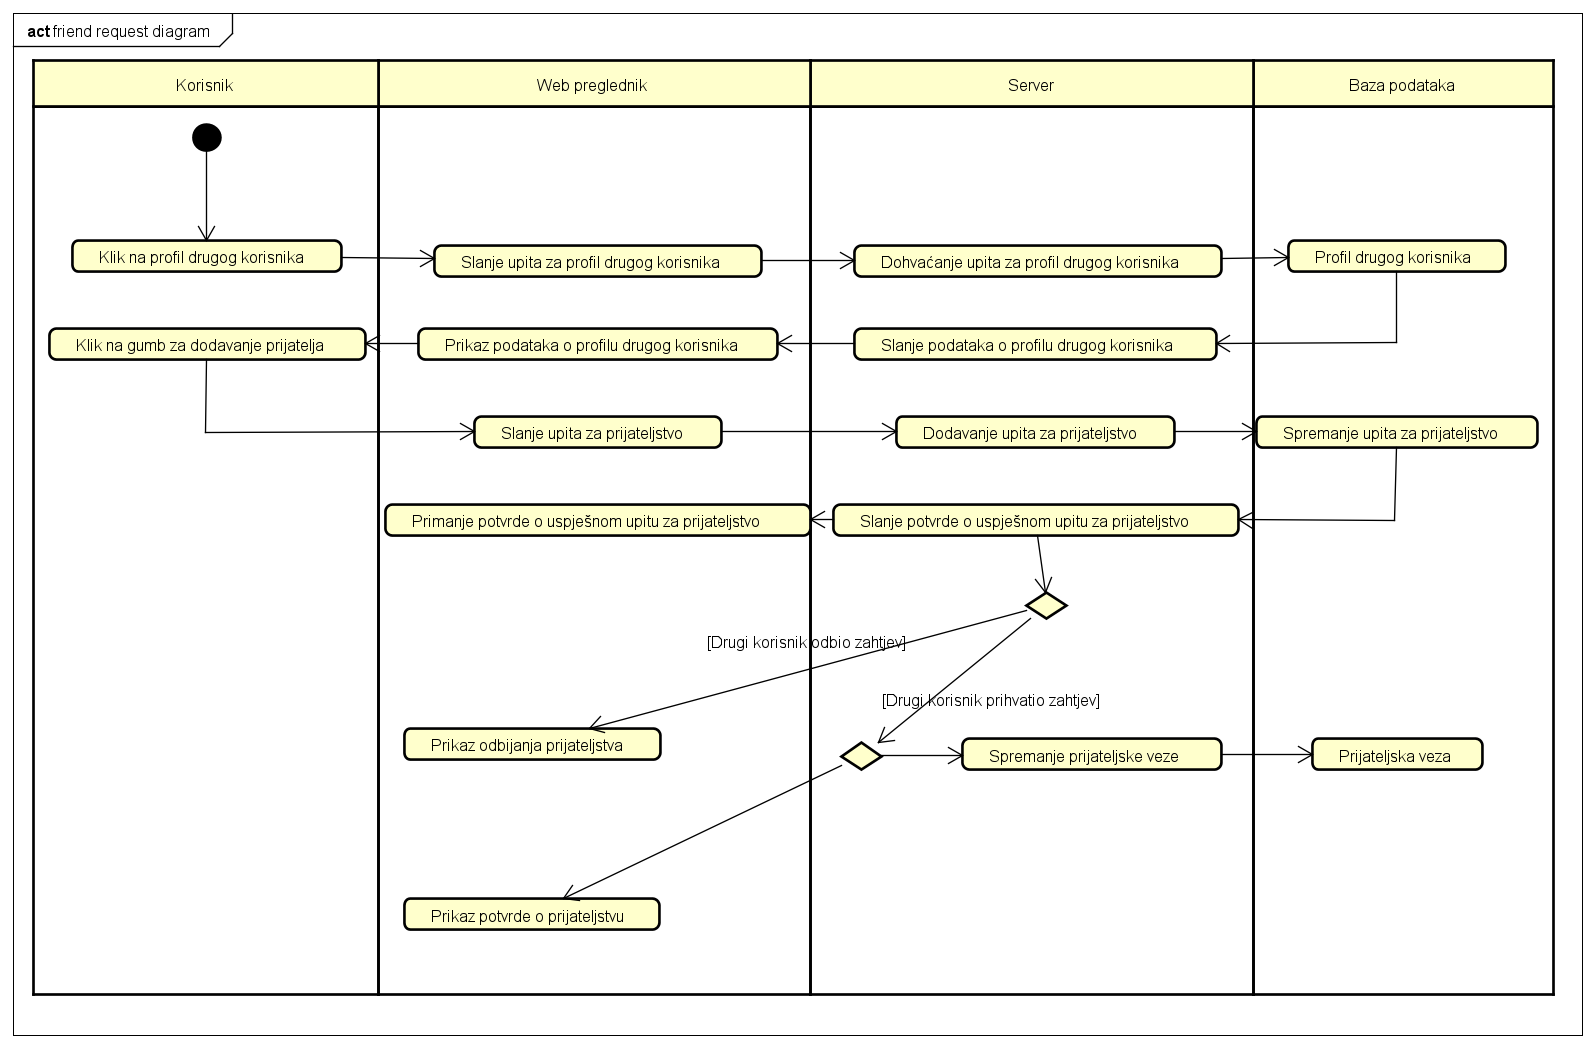
\includegraphics[scale=0.6, height=120mm, width=165mm]{dijagrami/activity/friend request diagram.png} %veličina slike u odnosu na originalnu datoteku i pozicija slike
		 	\centering
		 	\caption{Dijagram aktivnosti - dodavanje prijatelja}
		 	\label{fig:dijagrami_aktivnosti2}
			 \end{figure}
		 
		 	\begin{figure}[H]
		 	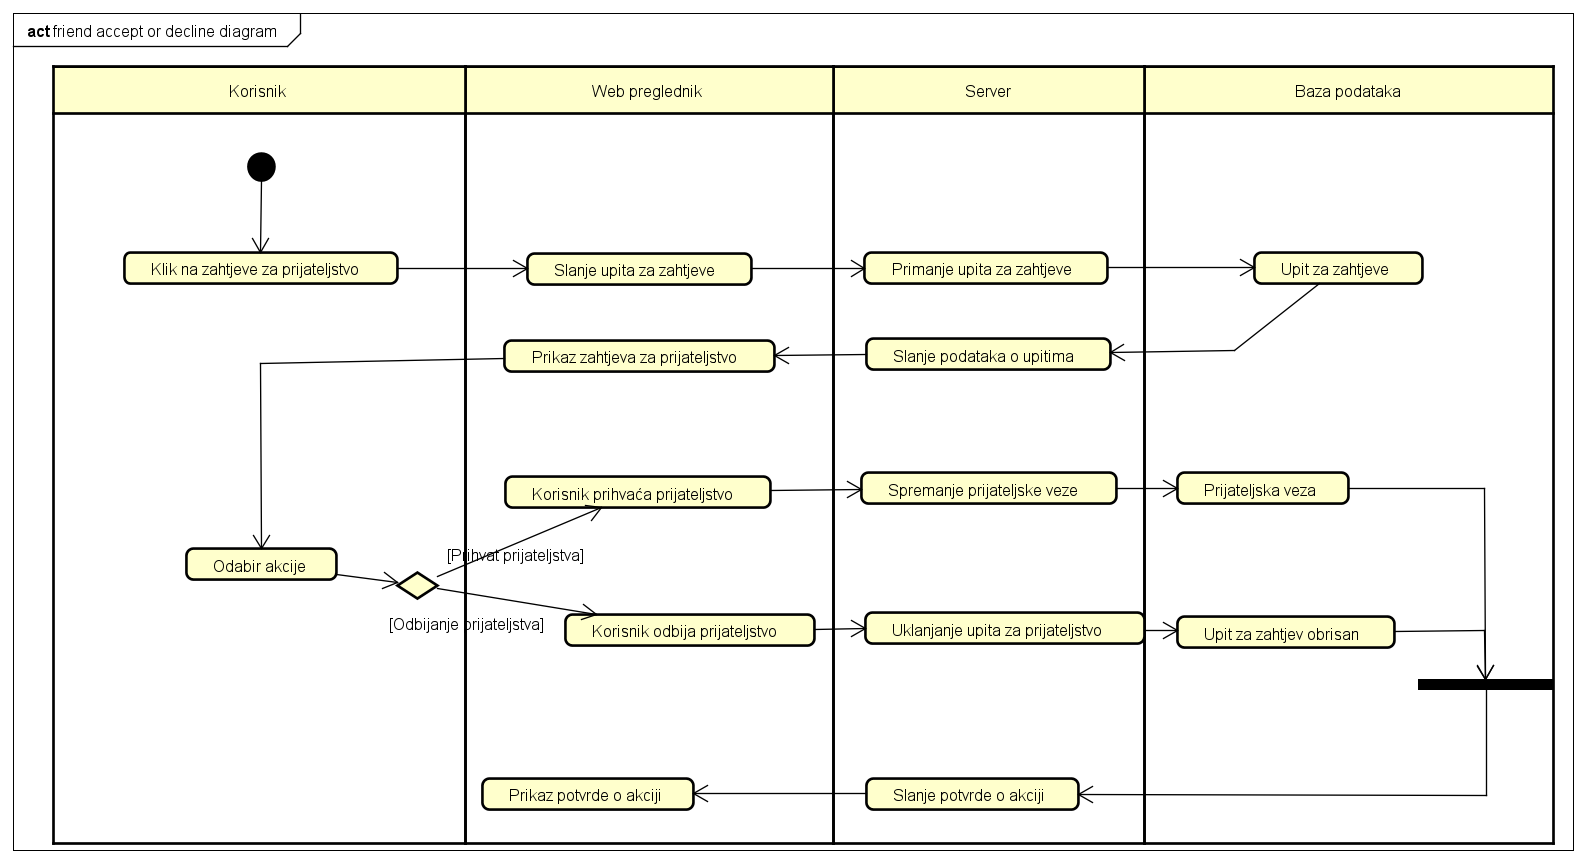
\includegraphics[scale=0.6, height=120mm, width=165mm]{dijagrami/activity/friend accept or decline diagram.png} %veličina slike u odnosu na originalnu datoteku i pozicija slike
		 	\centering
		 	\caption{Dijagram aktivnosti - prihvaćanje ili odbijanje prijateljstva}
		 	\label{fig:dijagrami_aktivnosti2}
		 	\end{figure}
			
		%	\eject
		%\section{Dijagram komponenti}
		
		%	\textbf{\textit{dio 2. revizije}}\\
		
		%	 \textit{Potrebno je priložiti dijagram komponenti s pripadajućim opisom. Dijagram komponenti treba prikazivati strukturu cijele aplikacije.}